% !TEX TS-program = xelatex
\documentclass[12pt,letterpaper]{article}

% ===========================
% HOUSE STYLE PREAMBLE
% ===========================
\usepackage{fontspec}

\setmainfont{EB Garamond}[
  Numbers=OldStyle,
  Ligatures=TeX,
]

% IPA fallback font
\newfontfamily\ipafont{Charis SIL}
\newcommand{\ipa}[1]{{\ipafont #1}}

% Lining figures when needed (tables, years in isolation)
\providecommand{\liningnums}[1]{{\addfontfeatures{Numbers=Lining}#1}}

% Monospace
\setmonofont{Inconsolata}[Scale=MatchLowercase]

% ===========================
% PAGE LAYOUT
% ===========================
\usepackage[
  letterpaper,
  inner=1.25in,
  outer=1in,
  top=1in,
  bottom=1.25in,
  marginparwidth=0.6in,
]{geometry}

\usepackage[british]{babel}
\usepackage[final]{microtype}

% ===========================
% HEADINGS
% ===========================
\usepackage{titlesec}

% Section: small caps, number in margin
\titleformat{\section}
  {\normalfont\scshape}
  {\llap{\thesection\quad}}
  {0pt}
  {}

% Subsection: small caps sentence case
\titleformat{\subsection}
  {\normalfont\scshape}
  {\thesubsection\quad}
  {0pt}
  {}

% Subsubsection: upright
\titleformat{\subsubsection}
  {\normalfont}
  {\thesubsubsection\quad}
  {0pt}
  {}

% Spacing
\titlespacing*{\section}{0pt}{2ex plus 1ex minus .2ex}{1ex plus .2ex}
\titlespacing*{\subsection}{0pt}{1.5ex plus 1ex minus .2ex}{0.5ex plus .2ex}
\titlespacing*{\subsubsection}{0pt}{1ex plus 0.5ex minus .1ex}{0.3ex plus .1ex}

% ===========================
% RUNNING HEADS
% ===========================
\usepackage{fancyhdr}
\pagestyle{fancy}
\fancyhf{}
\fancyhead[L]{\small\scshape\leftmark}
\fancyhead[R]{\small\thepage}
\fancyfoot{}
\setlength{\headheight}{13.6pt}
\setlength{\emergencystretch}{2em}
\addtolength{\topmargin}{-1.6pt}
\renewcommand{\headrulewidth}{0pt}

% ===========================
% COLORS & HYPERLINKS
% ===========================
\usepackage{xcolor}
\definecolor{linkmaroon}{RGB}{128, 0, 32}

\newif\ifanonymous
\ifdefined\anonymoussubmission
  \anonymoustrue
\else
  \anonymousfalse
\fi
\ifanonymous
  \newcommand{\pdfauthorfield}{}
\else
  \newcommand{\pdfauthorfield}{Brett Reynolds}
\fi

\usepackage{hyperref}
\hypersetup{
    colorlinks=true,
    linkcolor=linkmaroon,
    filecolor=linkmaroon,
    citecolor=linkmaroon,
    urlcolor=linkmaroon,
    pdftitle={Grammaticality de-idealized: Formal supplement},
    pdfauthor={\pdfauthorfield},
    pdfkeywords={grammaticality, projectibility, acceptability, preemption, entrenchment, conventionalization},
}
\usepackage{orcidlink}

% ===========================
% QUOTATIONS
% ===========================
\usepackage[style=american]{csquotes}
\MakeOuterQuote{"}

% ===========================
% SEMANTIC MACROS
% ===========================
\newcommand{\term}[1]{\textsc{#1}}
\newcommand{\mention}[1]{\textit{#1}}
\newcommand{\mentionh}[1]{⟨#1⟩}
\newcommand{\olang}[1]{\textit{#1}}
\newcommand{\abbr}[1]{\textsc{#1}}
\usepackage{marvosym}
\newcommand{\crossmark}{\textsubscript{\Cross}}
% ===========================
% MATHS AND SYMBOLS
% ===========================
\usepackage{amsmath,amssymb}

% ===========================
% LINGUISTIC EXAMPLES
% ===========================


% Judgement markers (TEXT-MODE SAFE)
\newcommand{\judgesep}{\kern-0.15em}
\newcommand{\ungram}[1]{*\judgesep#1}
\newcommand{\marg}[1]{\textsuperscript{?}\judgesep#1}
\newcommand{\odd}[1]{\#\judgesep#1}

% ===========================
% LISTS
% ===========================
\usepackage{enumitem}
\setlist{nosep, leftmargin=*}
\setlist[enumerate]{label=\arabic*.}
\setlist[itemize]{label=--}

% ===========================
% TABLES & FIGURES
% ===========================
\usepackage{booktabs}
\usepackage{array}
\usepackage{longtable}
\usepackage{float}
\usepackage{needspace}
\usepackage{graphicx}
\graphicspath{{figures/}}

% ===========================
% BIBLIOGRAPHY
% ===========================
\usepackage[backend=biber,style=apa,natbib=true,doi=true,isbn=false,url=true]{biblatex}
\addbibresource{refs.bib}

% Possessive citation
\newcommand{\posscite}[1]{\citeauthor{#1}'s (\citeyear{#1})}

% ===========================
% UTILITIES
% ===========================
\usepackage{xspace}
\newcommand{\eg}{e.g.\,\xspace}
\newcommand{\ie}{i.e.\,\xspace}
\newcommand{\etc}{etc.\xspace}

% ===========================
% DOCUMENT SPECIFIC PACKAGES
% ===========================
% Required for posterior plots
\usepackage{pgfplots}
\pgfplotsset{compat=1.18}
\usepgfplotslibrary{fillbetween}
\usepackage{tikz}
\usetikzlibrary{arrows.meta,shapes,positioning,fit,backgrounds}
\definecolor{lsLightGray}{RGB}{240,240,240}
\definecolor{lsMidBlue}{RGB}{0,114,178}
\usepackage{rotating}

% ===========================
% LINGUISTIC EXAMPLES (Must be last)
% ===========================
\usepackage{langsci-gb4e}
\makeatletter
\@ifundefined{noautomath}{}{\noautomath}
\makeatother


\usepackage{xr-hyper}
\externaldocument[M-]{grammaticality-de-idealized}

\title{Grammaticality de-idealized\\[0.4em]\large Formal supplement}
\ifanonymous
  \author{}
  \date{}
\else
  \author{Brett Reynolds \orcidlink{0000-0003-0073-7195}\\
    Humber Polytechnic \& University of Toronto\\
    \href{mailto:brett.reynolds@humber.ca}{brett.reynolds@humber.ca}}
  \date{\today}
\fi

\begin{document}
\maketitle

\begin{abstract}
This supplement gives the mathematical specification underlying the
Operator-Value Model of Grammaticality. It separates the population state from
speaker and analyst estimates, defines the observation and updating interfaces,
states the conditional population dynamics, records the simulation contract,
and maps the paper's structural claims to machine-checked Lean theorems. The
main paper presents the linguistic argument, predictions, and failure conditions
without formal notation. The supplement is designed to make every quantitative
commitment inspectable without making that notation a prerequisite for reading
the argument.
\end{abstract}

\noindent\textbf{Companion paper:} \emph{Grammaticality de-idealized}. Section
and example references that point outside this document refer to the main paper.

\tableofcontents
\newpage

\section*{Notation, types, and fixed parameters}
\addcontentsline{toc}{section}{Notation, types, and fixed parameters}
\label{sec:notation-register}

This register is part of the model specification. It states the type and role
of every recurring symbol before the derivations use it. A quantity called
\emph{fixed} is to be measured, normed, or registered independently of the
outcome it helps predict; it isn't silently fitted to that outcome. A quantity
called \emph{latent} is a world-side state inferred through an observation
model. A \emph{posterior} quantity belongs to a named epistemic bearer--speaker
or analyst--and can't be substituted for the corresponding latent state.

Several letters are overloaded only with explicit adornment or arguments. In
particular, $F$, $H$, $R$, $X$, $\pi$, and $\rho$ name distinct objects below;
$\ell_i$ is a lect, $\ell_j(x)$ and $\ell^{\mathrm{omit}}_{i,t}(x)$ are
omission diagnostics, and $\ell(k)$ is a locality function; $d$ can index an
operator dimension or dependency while
$d_j$ is an omission contrast; $c$ is a conditioning state while $c_k$ is a
mixture coefficient; and $r$ can be an epistemic bearer while $r_j$ and
$r(\Delta,\iota)$ are attribution and repair functions. The table flags each
use. Time is discrete except in the optional cubic normal form. All
probabilities and rates lie in $[0,1]$ unless stated otherwise.

\footnotesize
\begin{longtable}{@{}>{\raggedright\arraybackslash}p{0.18\textwidth}
  >{\raggedright\arraybackslash}p{0.25\textwidth}
  >{\raggedright\arraybackslash}p{0.48\textwidth}@{}}
\toprule
Symbol & Type or domain & Meaning and status \\
\midrule
\endfirsthead
\toprule
Symbol & Type or domain & Meaning and status \\
\midrule
\endhead
\midrule
\multicolumn{3}{r}{\emph{continued on next page}}\\
\endfoot
\bottomrule
\endlastfoot

\multicolumn{3}{@{}l}{\textsc{Indices, bearers, and linguistic objects}}\\[2pt]
$t,s,t_0$ & discrete times & Current time, a time inside a window, and the independently fixed initial time. \\
$W_t=[t-W,t)$ & finite time window & Preceding convention-individuating window of fixed width $W$. \\
$i,j$ & speakers & $i$ usually marks the focal speaker; $j$ indexes a sampled population member or observation. \\
$r\in\{i,a\}$ & epistemic bearer & A speaker $i$ or analyst $a$ whose evidence licenses a posterior estimate. \\
$c\in\mathcal C$ & conditioning state & Construed communicative situation and norm centre; $\mathcal C$ is its state space. \\
$n$ & niche identifier & Independently specified communicative job. \\
$\phi,\varphi(A)$ & frame type, frame function & Constructional frame and the frame type of assembly $A$, used to type zero-marking alternatives and obligatoriness. \\
$d$ & operator dimension & A community-indexed contrast dimension; not an exponent. \\
$f,v,u$ & form, value, token & $f$ is a form, $v$ its intended value, and $u$ a token notation used only when $v$ is recoverable. \\
$x,x',y$ & candidate realizations & Form--value candidates in a niche; $y$ is the observed choice. \\
$\kappa$ & constructional node & Licensing-bearing identity of a typed construction or sign. \\
$A$ & finite assembly & Complete typed assembly of constructions; its linguistic representation may be richer than the fields projected into the model. \\
$\ell_i$ & lect state & Latent lect component for speaker $i$; $H$ is the finite number of lect components. \\

\multicolumn{3}{@{}l}{\textsc{Constraint structure and state theory}}\\[2pt]
$O(c)$ & finite dimension set & Operator dimensions conventionalized for conditioning state $c$; examples in the text are illustrative, not exhaustive. \\
$\Omega$ & typed constraint space & Space in which partial operator contributions can refine or conflict. \\
$\omega_\kappa,\omega(A)$ & partial constraints & Operator contribution of node $\kappa$ and the unified contribution of assembly $A$. \\
$\sqcup,\bot$ & partial join, failure & Constraint unification and undefined/inconsistent result. The same glyph $\bot$ later denotes the typed outside option when it appears as a choice argument. \\
$\mathcal H$ & construction hierarchy & Independently specified inheritance structure that generates analogical candidates. \\
$\mathcal A(f,v)$ & finite assembly set & Complete assemblies with yield $f$ and value $v$. \\
$\mathcal A_0(d,n,\phi,c)$ & finite assembly class & Independently fixed defined assemblies that realize niche $n$ in frame $\phi$ while leaving dimension $d$ unset. \\
$\operatorname{def}(A)$ & Boolean predicate & Whether the operator constraints in $A$ unify. \\
$\operatorname{sat}_t(A,c)$ & Boolean predicate & Whether $A$ supplies every dimension that the prior population history makes obligatory. \\
$\mathrm{OBL}_t(n,c,\phi)$ & dimension set & Path-dependent ontic obligatoriness macro, determined from prior realized population behaviour and prior convention state. \\
$z_{i,t}(\kappa,c)$ & binary latent state & Whether speaker $i$ includes construction $\kappa$ in the repertoire for $c$ at $t$. \\
$Z_t(\kappa,c)$ & predictive binary state & Inclusion of a newly sampled exchangeable speaker, conditional on population parameters. \\
$\theta_t(\kappa,c)$ & latent population rate & Exchangeable population licensing rate for construction $\kappa$. \\
$\boldsymbol\pi$ & simplex vector & Lect-mixture weights; distinct from the usage rate $\pi_t$ below. \\
$L_t(A,c)$ & predictive event & A sampled speaker includes every node required by $A$. \\
$\Lambda_{i,t}$ & state vector & Speaker $i$'s vector of constructional inclusion states. \\
$S_t^\theta(f,v,c)$ & latent population state & Prevalence of at least one defined, saturated, licensed assembly route. \\
$\mathcal Y_{W_t}$ & population history & Realization rates, pressure statistics, and prior obligatoriness state in the preceding window. \\
$\mathcal D_{r,t}$ & bearer evidence & Evidence available to bearer $r$ through time $t$. \\
$\widehat S_t^{(r)}$ & posterior mean & Bearer $r$'s estimate of the population status state. \\
$G_t,g_{i,t}$ & posterior means & Compact names for the analyst's and speaker $i$'s status estimates. \\
$C_t^{(r)},\widehat C_t$ & posterior means & Bearer-specific and analyst means for a pivotal construction's licensing rate. \\
$\nu_t^{(r)},\widehat\nu_t$ & positive concentrations & Evidence concentration for the corresponding posterior estimate. \\
$U_{\mathrm{epi}}^{(r)}$ & posterior variance & Epistemic uncertainty about the population state for bearer $r$. \\
$U_{\mathrm{het}}^{(r)}$ & expected Bernoulli variance & Predicted between-speaker heterogeneity; not posterior uncertainty. \\
$\tau(c)$ & fixed decision parameter & Situation-specific read-out boundary determined by losses; not part of constitutive status. \\

\multicolumn{3}{@{}l}{\textsc{Opportunity, choice, and observation}}\\[2pt]
$\mathcal V_{n,t}^{\star}$ & finite candidate set & Attested, hierarchically constructible, and analogically generated candidates for niche $n$; the star marks inclusion of zero-token candidates. \\
$N_t(n,c)$ & non-negative count & Opportunities for niche $n$ in state $c$ during the current window. \\
$k_t(x,n,c)$ & non-negative count & Observed choices of candidate $x$ in that window. \\
$U_t(x;n,c)$ & real utility & Population-level counterfactual choice utility. \\
$U_{i,t}(u;n,c)$ & real utility & Speaker-specific counterpart of the choice utility. \\
$\mathbf f,\mathbf w$ & feature vector, weights & Choice predictors and their fixed or independently estimated coefficients. \\
$\bot$ & outside-option realization & Avoidance, periphrasis, silence, or repair in progress; typed separately from constraint failure. \\
$\rho_t^\star$ & candidate-only probability & Counterfactual share when every registered candidate is available and the outside option is omitted. \\
$\widetilde\rho_t^\star$ & full-choice probability & Counterfactual share when the outside option is included; it enters the licensing--choice approximation. \\
$\pi_t(x\mid n,c)$ & latent usage rate & Population probability of producing candidate $x$ in the niche; distinct from lect weights $\boldsymbol\pi$. \\
$r_j$ & attribution probability & Independently coded probability that occasion $j$ is genuinely an opportunity for the target. \\
$\ell_j(x)$ & log likelihood ratio & Information diagnostic comparing an observed non-target choice under target absence and presence. \\
$\ell^{\mathrm{omit}}_{i,t}(x)$ & log likelihood ratio & Speaker-indexed normalized-softmax omission diagnostic for target $x$. \\
$d_j$ & probability contrast & Attribution-weighted omission informativeness used in the likelihood. \\
$s_t,m_t$ & current-window counts & Target choices and non-target choices entering the current update exactly once. \\
$a_t,b_t$ & positive filter shapes & Parameters of the bearer-specific Beta approximation. \\
$a^0,b^0$ & fixed positive shapes & Baseline prior parameters. \\
$\widetilde a_t,\widetilde b_t$ & discounted shapes & Accumulated evidence after discounting and before the current window. \\
$\delta_m$ & fixed memory parameter & Retention of accumulated evidence; one means no forgetting. \\
$c_k$ & non-negative coefficient & Bernstein-expansion coefficient for the affine omission product. \\
$\mu_{t+1},v_{t+1}$ & exact moments & Mean and variance of the finite Beta mixture before moment projection. \\
$\lambda_{i,\kappa}$ & fixed persistence weight & Rate at which evidence can alter speaker $i$'s next inclusion state. \\
$h_\kappa$ & adoption response & Independently specified probability of adoption or retention from evidence and covariates. \\
$q_\kappa$ & fixed adoption criterion & Switching or coordination cost used by the posterior-threshold response. \\
$\xi_{i,t}$ & covariate vector & Independently specified lect, network, cohort, and adoption covariates. \\
$M$ & positive integer & Finite population size; distinct from anomaly drive $M_{i,t}$ below. \\
$\theta_t^{(M)}$ & empirical finite-population rate & Realized proportion of the $M$ speakers who include the focal construction. \\
$D_{0,i}$ & positive normalizer & Gated full-choice denominator when the target is unavailable. \\

\multicolumn{3}{@{}l}{\textsc{Repair, read-out, and situation inference}}\\[2pt]
$\Delta(d)$ & non-negative divergence & Expected change to the common-ground posterior when operator dimension $d$ is mis-set; estimated from independent comprehension probes. \\
$\iota$ & footing covariates & Interactional factors conditioning repair. \\
$r_{\mathrm{upd}},r_{\mathrm{form}}$ & repair probabilities & Update-oriented repair and value-intact form correction. \\
$r(\Delta,\iota)$ & repair response & Generic repair-targeting response to update divergence and footing. \\
$\sigma$ & logistic link & Link used in the speaker-level repair read-out. \\
$\eta_0,\eta_1$ & real coefficients & Repair-read-out intercept and positive sensitivity to estimated non-licensing. \\
$\psi_{\mathrm{upd}},\psi_{\mathrm{form}}$ & expected exposures & Window-level update-oriented and form-oriented repair opportunities. \\
$e$ & observed situation cues & Evidence from which a hearer infers the conditioning state. \\
$q_h(c\mid e)$ & hearer posterior & Hearer $h$'s situation ascription given cues. \\
$R_i(u,e)$ & non-negative cost vector & Processing, recovery, surprisal, and plausibility costs after situation uncertainty is integrated. \\
$I_i(u,e)$ & non-negative scalar & Prescriptive or ideological dissonance. \\
$M_{i,t}$ & real anomaly drive & Weighted combination of low expected status, implementation costs, dissonance, and noise. \\
$F_{i,t}$ & value in $(-1,0]$ & Bounded signed anomaly read-out; distinct from the population map $F$ below. \\
$\alpha_G,\boldsymbol\gamma,\delta_I$ & fixed read-out weights & Contributions of expected status, implementation costs, and dissonance. \\
$\varepsilon_i$ & noise term & Speaker-level residual in the anomaly read-out. \\
$\mathcal L_{\mathrm{loc}}$ & non-negative cost & Dependency-locality component of implementation cost. \\
$\mathcal D_{\mathrm{dep}},|d|$ & dependency set, length & Dependencies in a token and the registered length of each. \\
$K_{\mathrm{sat}},\beta_L,\eta_L$ & fixed locality parameters & Saturation point, scale, and sublinear exponent for long dependencies. \\
$\Phi^{\mathrm{ev}},\Phi^{\mathrm{dec}}$ & confidence read-outs & Evidence confidence and confidence in a binary decision. \\
$\nu_0$ & positive scale & Fixed concentration scale in evidence confidence. \\
$\zeta$ & attribution category & Inferred source of anomaly: local non-licensing, other community, speaker error, noise, or own overload. \\

\multicolumn{3}{@{}l}{\textsc{Population dynamics and obligatoriness}}\\[2pt]
$X_t=(\theta_t,a_t,b_t)$ & coupled state & Population rate and evidence-filter shapes for the focal candidate. \\
$\mathcal M_\theta$ & deterministic operator & Expected-window likelihood update holding the population rate fixed. \\
$F(X_t)$ & deterministic map & Composed mean-field population-and-evidence transition; distinct from anomaly $F_{i,t}$. \\
$J_F$ & Jacobian matrix & Local linearization of the full map. \\
$\rho(J_F)$ & spectral radius & Stability diagnostic; unrelated to the choice shares bearing a star. \\
$H(\theta)$ & scalar crossing function & Adoption response after the evidence state is allowed to settle at fixed population rate. \\
$\theta^\ddagger$ & interior boundary & Population coordinate of the unstable basin boundary in the declared numerical regime. \\
$\alpha,\beta$ & positive constants & Coefficients of the optional cubic normal form only. \\
$R_s^0(A,n,c)$ & realized population rate & Raw zero-marking rate; neither licensing nor an analyst estimate. \\
$\Pi_{W_t}$ & realized pressure & Attributable marked-competitor pressure in the preceding window, weighted by full-choice shares and excluding outside-option choices. \\
$E_t,X_t$ & Boolean conditions & Entry and release conditions for obligatoriness; the argument list distinguishes release $X_t$ from the coupled state above. \\
$\epsilon_0,\epsilon_1$ & registered rate thresholds & Entry and release cutoffs with the release threshold strictly higher. \\
$\pi_0,\pi_1$ & registered pressure thresholds & Entry and release cutoffs with the release threshold strictly lower. \\
$\nu_{\min}$ & registered evidence floor & Minimum effective concentration for an analyst to identify obligatoriness; it warrants an ontic claim but doesn't constitute it. \\
\end{longtable}
\normalsize

Local quantities used for a single equation are defined immediately before or
after that equation. If a recurring symbol isn't in this register and lacks a
local definition, that absence is a specification error rather than an
invitation to infer its meaning from convention.


\section{A formal core: grammaticality as conditioned stability}
\label{sec:formalism}

The framework separates two explanatory targets. A \term{state theory} specifies
the conditions under which a form--value pair is grammatical \emph{for a
population in a communicative situation} at time $t$; a \term{dynamics module}
specifies candidate routes by which such states arise, persist, and change.

The distinction matters because the account is projectibility-first. Its
primary payoff is a family of inferences: observing part of a grammaticality
profile should license expectations about repair, transmission, exposure, and
change in cases not used to define the profile. The state theory specifies the
world-side pattern over which those projections run. The dynamics module then
states candidate \term{support} hypotheses about what could stabilize that
pattern and, where the evidence warrants, maintain it. Support claims come in
grades.
Stabilization, maintenance by a production--repair loop, and control by a
deviation-detecting process are distinct claims, each requiring independent
evidence \autocite{reynolds2026kindsProjectibilityProfiles,
reynolds2026notEveryStableCluster}.
In Woodward's interventionist terms, a stabilizer earns that status when an intervention on it changes the profile in an invariant, predictable way \autocite{woodward2003MakingThingsHappen, woodward2001}.

\subsection{Conditioning structure}
\label{sec:conditioning}

Let $c\in\mathcal{C}$ be a \term{conditioning state}, a construed communicative situation in \posscite{wiese2023} sense, together with whatever norm-centre is treated as relevant. Nothing here requires $c$ to be externally given; interlocutors can misalign about $c$, and $c$ can be learned, split, and renegotiated over time.

For many purposes it helps to think of $c$ as a bundle that may include situational features (activity type, medium, footing), stable baselines tied to speaker ascription, and norm-orientation (discourse-community identification), but the formalism treats $c$ abstractly as the conditioning variable that selects the relevant distribution of form--value relations.

\Needspace{17\baselineskip}
\subsection{Objects}
\label{sec:objects}

Before introducing the notation, here is the ordinary-language picture. An
assembly is a candidate way of building a form--value pair out of learned
patterns. The model asks four questions about it: is there a way to build it at
all? Do the grammatical instructions contributed by its parts fit together? Are
the instructions that this situation requires actually supplied? And does the
relevant community treat the patterns involved as available resources? A
negative answer can arise at any of these points. Difficulty of processing,
implausibility of the construal, and prescriptive dissonance are different: they
can make an otherwise licensed assembly feel bad without changing its status.

The table maps that sequence onto the formal core. The prose that follows first
describes constructions and assemblies, then distinguishes the community state
from the evidence-based estimate of it. Readers need not retain the symbols on
first pass: grammatical status tracks whether a population has an assembly that
passes all four questions in a situation, while the evidence also records how
settled that estimate is.

\begin{table}[htbp]
\centering
\small
\begin{tabular}{@{}>{\raggedright\arraybackslash}p{0.21\textwidth}
  >{\raggedright\arraybackslash}p{0.28\textwidth}
  >{\raggedright\arraybackslash}p{0.38\textwidth}@{}}
\toprule
Expository role & Formal object (\S3) & Work in the formal core \\
\midrule
coverage / structural viability & $\mathbf{1}\bigl[\mathcal{A}(f,v)\neq\emptyset\bigr]$ &
  structural viability: some covering assembly exists \\
operator compatibility & $\operatorname{def}(A)$: unification &
  hard operator-value compatibility \\
saturation & $\operatorname{sat}_t(A,c)$ &
  derived saturation of obligatory dimensions \\
content oddness & plausibility term in $R_i$ (\S\ref{sec:feeling-new}) &
  content-oddness as a subjective cost \\
situational licensing & population rate $\theta_t$; Beta posterior; $L_t(A,c)$ &
  population licensing and its evidence state \\
status profile & $S_t^{\theta}$ population state;
  $\widehat{S}^{(r)}_t=\mathbb{E}_r[S_t^{\theta}]$ &
  status and its epistemic estimate; simple products are limiting cases
  (\S\ref{sec:posterior-existence}) \\
decision threshold & $\tau(c)$, \S\ref{sec:decision-readout} & decision-theoretic read-out only \\
\bottomrule
\end{tabular}
\caption{Where the expository roles from the opening sections live in the formal core. The formal implementation uses assemblies, unification, licensing posteriors, and decision read-outs.}
\label{tab:notation-bridge}
\end{table}

The typed notation register preceding this section defines every recurring
symbol and fixed parameter. Local quantities that occur in only one derivation
are defined where they enter. The register is authoritative when a familiar
letter has more than one explicitly marked role.

The core's linguistic unit is the construction, in the CxG sense of a learned
typed association at any grain \citep{fillmore1988,
goldberg1995constructions,sag2012sign}. Following the richer Sign-Based
Construction Grammar perspective, a construction can constrain phonology,
syntax, semantics, discourse context, and relations among daughter signs. This
richer object isn't reducible to a bare form--meaning pair. The quantitative model
uses a task-specific projection of that richer object: a typed form template,
content contribution, partial operator constraint $\omega_\kappa$, frame and
niche tags, and a constructional identity $\kappa$ on which licensing is
defined. Any additional SBCG fields remain available to the coverage and typing
system even when the statistical dynamics don't inspect them. Nothing here is
level-specific: a construction can be the plural cell of a lexeme, a clause
pattern, an intonational contour, or a code-mixed frame.

Operator contributions live in a typed constraint space $\Omega$ over a
dimension set $O(c)$. Illustrative dimensions are clause type, polarity,
tense--aspect anchoring, role allocation, scope, reference tracking, and
information-packaging instructions; this isn't an exhaustive inventory. Which
dimensions belong to $O(c)$ is itself
conventional: a contrast enters only when the community has conventionalized it
as an operator contrast in the sense of \S\ref{M-sec:operator-values}, so the
inventory is community-indexed. Atomic feature--value assignments are a useful
special case, but the general object is a constraint structure: tense intervals,
scope relations, anaphoric dependencies, and information-packaging requirements
can refine one another without being identical atomic values. Two contributions
\term{unify}, written $\omega \sqcup \omega'$, iff their conjunction is
satisfiable in the typed constraint system; otherwise the join is undefined
($\bot$). Compatibility remains Boolean, but equality of atomic values isn't
the only way to satisfy it.

An \term{assembly} $A$ is a finite tree of constructions with all slots filled. Its yield is $\mathrm{form}(A)$; its operator assignment is $\omega(A)=\bigsqcup_{\kappa\in A}\omega_\kappa$, defined iff all contributions unify; its value is $\mathrm{val}(A)$. Three predicates over assemblies do the core work:

\begin{align}
\operatorname{def}(A) &= \mathbf{1}\bigl[\omega(A)\ \text{is defined}\bigr]
  && \text{(compatibility)} \\
\operatorname{sat}_t(A,c) &= \mathbf{1}\bigl[\omega(A)\ \text{is total on}\
  \mathrm{OBL}_t(n(A,c),c,A)\bigr]
  && \text{(saturation)} \\
L_t(A,c) &= \textstyle\bigwedge_{\kappa\in A} Z_t(\kappa,c)
  && \text{(licensing)}
\end{align}

Compatibility is hard: there's no weighting an operator clash away. Saturation
refers to the obligatory dimensions $\mathrm{OBL}_t(n(A,c),c,A)$, which aren't
stipulated per language. Section~\ref{sec:derived-obligatoriness} derives them
from a preceding window of population-level, niche-specific zero-marking rates
and ungated preemption pressure, without using the analyst's posterior or
saturation itself.
On this definition, $\operatorname{sat}_t$ is a path-dependent ontic macro rather than an
independent primitive or an epistemic estimate. For an assembly $A$ of frame
type $\varphi(A)$ and registered at-issue niche $n(A,c)$,
$\mathrm{OBL}_t(n(A,c),c,A)$ abbreviates
$\mathrm{OBL}_t(n(A,c),c,\varphi(A))$. English progressive marking and Turkish
evidential marking are the worked cases there.

Licensing is latent, and the Beta is typed over a rate rather than a fixed binary
fact. Let $z_{j,t}(\kappa,c)\in\{0,1\}$ be speaker $j$'s local inclusion state
for construction $\kappa$ in $c$. The population state
$\theta_t(\kappa,c)\in[0,1]$ is the latent exchangeable licensing-rate
parameter. For a randomly sampled exchangeable speaker,
$Z_t(\kappa,c)\mid\theta_t(\kappa,c)\sim
\mathrm{Bernoulli}(\theta_t(\kappa,c))$ is the predictive inclusion state for
that speaker, and $L_t(A,c)$ is the event that the sampled speaker licenses all
nodes in $A$. The definition needs a joint predictive distribution
over the vector $\{Z_t(\kappa,c):\kappa\in A\}$. Posterior dependence among
node rates represents epistemic co-uncertainty; it doesn't by itself generate
co-licensing within a speaker. A tractable joint model introduces a latent lect
$\ell_i\in\{1,\ldots,H\}$ for speaker $i$:
\[
\ell_i\sim\mathrm{Categorical}(\boldsymbol{\pi}),\qquad
z_{i,t}(\kappa,c)\mid\ell_i=\ell\sim
\mathrm{Bernoulli}\!\left(\theta_{\ell,t}(\kappa,c)\right).
\]
Conditional independence across nodes within a lect is still an approximation;
an explicit within-lect joint can replace it where constructional kin cluster
more tightly. Under this tractable version,
\[
P\!\left(L_t(A,c)=1\mid\boldsymbol{\pi},\boldsymbol{\theta}_t\right)=
\sum_{\ell=1}^{H}\pi_\ell\prod_{\kappa\in A}
\theta_{\ell,t}(\kappa,c),
\]
and the marginal rate used elsewhere is
$\theta_t(\kappa,c)=\sum_\ell\pi_\ell\theta_{\ell,t}(\kappa,c)$. The
independent product of marginal node rates is a single-lect limiting
case, not a general account of assembly prevalence.

No speaker or analyst observes $\theta$ directly. Under exchangeability, de Finetti's
representation theorem supplies a mixing measure over $\theta$
\citep{deFinetti1937}. The Beta family is the conjugate specialization
that adds linear predictive updating: in the Bernoulli case, linearity of the
posterior expectation of success in the counts is the binary analogue of
Johnson's sufficientness postulate in Zabell's generalization
\citep{zabell1982}. Direct inclusion observations would preserve that
conjugacy. The choice observations used here don't: a non-target choice has an
affine likelihood in $\theta$, so its exact finite-window posterior is a Beta
mixture. Section~\ref{sec:update} uses the Beta family as an
assumed-density approximation, matching the exact mixture's mean and variance
after each window. A speaker's filter has mean
$C^{(i)}_t(\kappa,c)$ and concentration $\nu^{(i)}_t(\kappa,c)$; an analyst can
use the same family with a different evidence set, producing
$\widehat C_t$ and $\widehat\nu_t$. The choice likelihood, memory discount, and
moment projection are distinct modelling commitments. The population
transition in~\eqref{eq:inclusion-transition} states how speakers' filters can
alter later inclusion; updating an analyst posterior doesn't alter the
population. The vector $\Lambda_{i,t}$ collects speaker $i$'s inclusion states
$z_{i,t}(\kappa,c)$, and the population distribution over those vectors supplies
the population-level status state.

Compositional inheritance matters here. A novel token such as \mention{She
texted him the address} needn't have been encountered: the assemblies covering it
are built from nodes--ditransitive transfer, pronominal object order, the relevant
lexical-category relations--each with its own posterior, and the token inherits its
status through them. What the learner updates is constructional regions, not
memorized sentence types, so first-heard sentences aren't predicted to have zero
licensing. Actual statistical pooling would require hierarchical hyperpriors
over construction families, lexemes, and situations; this core needs only
the compositional inheritance just described.

\subsection{Grammatical status as a conditioned state property}
\label{sec:objective-G}

\subsubsection{Status and its posterior estimate}
\label{sec:posterior-existence}

For a form $f$, value $v$, and conditioning state $c$, let $\mathcal{A}(f,v)$ be
the set of assemblies with yield $f$ and value $v$, and let
$\mathcal Y_{W_t}$ collect the preceding window's population realization rates,
ungated pressure statistics, and prior obligatoriness state. The population
state is

\begin{equation}
S_t^{\theta}(f,v,c)=
P\Bigl(\,\exists A\in\mathcal{A}(f,v):\;
\operatorname{def}(A)\wedge\operatorname{sat}_t(A,c)\wedge L_t(A,c)
\,\Bigm|\,\boldsymbol{\theta}_t,\mathcal Y_{W_t},c\Bigr),
\label{eq:Gtheta}
\end{equation}

\noindent the prevalence, among exchangeable speakers in $c$, of at least one
defined, saturated, licensed route to the form--value pair. The history argument
is needed because $\operatorname{sat}_t$ inherits its path dependence from
$\mathrm{OBL}_t$, which is determined
by the preceding population window and prior convention state rather than by an
instantaneous estimate.
Neither a learner nor an analyst observes this population state directly. For
an epistemic bearer $r$ (a speaker $i$ or an analyst $a$), the estimate is

\begin{equation}
\widehat{S}^{(r)}_t(f,v,c)=
\mathbb{E}_{p_r(\boldsymbol{\theta}_t,\mathcal Y_{W_t}\mid\mathcal{D}_{r,t})}
\!\left[S_t^{\theta}(f,v,c)\right],
\label{eq:Gt}
\end{equation}

\noindent where $\mathcal{D}_{r,t}$ is that bearer's evidence to date: tokens,
structured omissions, repairs, avoidance, and situation cues. Status is the
population property $S_t^{\theta}$; $\widehat{S}^{(r)}_t$ is a particular
bearer's estimate of it. For compactness, later predictive equations write
$G_t$ for the analyst's $\widehat{S}^{(a)}_t$ and $g_{i,t}$ for speaker $i$'s
$\widehat{S}^{(i)}_t$. Where
value is recoverable from context, I write $G_t(u,c)$ and $S_t^{\theta}(u,c)$
for readability. For a single pivotal node,
$S_t^{\theta}=\theta_t(\kappa,c)$ when compatibility and saturation are fixed at
one, so the estimate's mean and concentration are literally the corresponding
Beta posterior's mean and concentration.

Two scope conditions matter. First, for a finite yield and a finite,
non-empty-recursive construction inventory (no cycles of null-yield
expansions--the standard offline-parsability condition), $\mathcal{A}(f,v)$ is
finite, so the existential is a finite disjunction. No additional tractability
stipulation is needed.

Second, the relation to simpler heuristics. In the high-precision limit, where
every node posterior has concentrated, the pair~\eqref{eq:Gtheta}--\eqref{eq:Gt}
has the same limiting
classification as a weakest-link rule over the best assembly: a licensed,
defined, saturated assembly exists or it doesn't. And under a single-lect,
within-speaker node-independence approximation, posterior independence across
nodes, and a single dominant assembly $A^{\ast}$, the mean factorizes,

\begin{equation}
\widehat{S}^{(r)}_t(f,v,c)\approx \mathbf{1}\bigl[\operatorname{def}(A^{\ast})\bigr]
\cdot \mathbf{1}\bigl[\operatorname{sat}_t(A^{\ast},c)\bigr]
\cdot \prod_{\kappa\in A^{\ast}} C_t(\kappa,c).
\end{equation}

\noindent A three-factor product heuristic can work in easy cases as the
single-assembly, independent, high-precision special case
of~\eqref{eq:Gtheta}--\eqref{eq:Gt}, with structural viability as non-emptiness and
hard compatibility folded into $\operatorname{def}$. Away from that
limit,~\eqref{eq:Gtheta} supplies the population state and~\eqref{eq:Gt} its posterior
mean, so uncertainty remains part of the status profile rather than being folded
into the mean.

A three-factor heuristic can also hide content-oddness inside compatibility--the
concentration of construal for cases like \mention{colorless green ideas}. That
work lives instead in the subjective read-out's cost vector
(\S\ref{sec:feeling-new}). A lexically bizarre but operator-compatible construal
doesn't lower $S_t^{\theta}$ or its estimate and shows up as a plausibility
cost in $R_i$: the sentence is grammatical and odd, matching the target
contrast.

\subsubsection{Projectible use of the posterior state}
\label{sec:projectible-use}
\label{sec:projectible-G}

Grammaticality projects over this posterior state. $G_t$ is compact notation for
the analyst's estimate $\widehat{S}^{(a)}_t$, the mean of a posterior random
variable whose dispersion remains available for projection.
Figure~\ref{fig:state-space} depicts both the estimate and its
dispersion.

The causal bearers remain speakers and their inclusion or evidence states. A
speaker's candidate availability gates production, while a hearer's own estimate
$g_{i,t}$ can enter repair:

\begin{align}
\Pr_i(\text{produce }u\mid n,c,t) &\propto
  z_i(u,c)e^{U_{i,t}(u;n,c)}, \\
\Pr_i(\text{repair }u\mid c,t) &=
  \sigma\!\left(\eta_0+\eta_1
  \bigl(1-g_{i,t}(u,c)\bigr)\,r(\Delta,\iota)\right), \qquad \eta_1>0,
\end{align}
\noindent where $z_i(u,c)$ abbreviates availability of a complete route for
speaker $i$ (expanded in \S\ref{sec:usage}) and $\sigma$ is the logistic link.

\noindent The repair expression is the $\Delta$-sensitive form used in
\S\ref{sec:repair-controller}; if $\Delta$ and footing are marginalized out, it
reduces to a monotone reduced form in $1-g_{i,t}$. Aggregate production and
repair are obtained by integrating over speakers; $G_t$ predicts those rates but
doesn't cause them. This scopes the controller claim:
licensing failures with readily recoverable intended updates but low update divergence should attract only
baseline understanding-repair and, if stable, be supported mainly by preemption, while
operator mis-settings draw the $\Delta$-scaled repair flow; correction rates
should instead track ascription and prescriptive dissonance.

Other generalizations run over epistemic concentration, and they're the
diagnostic ones. Two form--value pairs can share a low mean while differing in
how much evidence backs it, and the update dynamics make them behave differently
under new exposure: a diffuse posterior moves with framing and familiarization;
a concentrated one doesn't. This epistemic dispersion is
$\operatorname{Var}(S_t^{\theta}\mid\mathcal{D}_{r,t})$ for epistemic bearer
$r$. Behavioral predictions use a speaker's $r=i$ posterior; analyst-facing
estimates use $r=a$. In single-node cases the corresponding concentration is
the pivotal node's $\nu^{(r)}$.

Population heterogeneity is different. A community can have a sharply estimated
interior $\theta$ because speakers are genuinely split, as with \mention{might
could} in a mixed community. That state has low epistemic variance but high
between-speaker disagreement. The interior estimate counts as genuine
heterogeneity only when no independently specifiable refinement of $c$
(\S\ref{sec:identification-c}) splits the population toward the attractors; if
such a partition exists, the apparent heterogeneity was a mis-specified
conditioning state. Within-speaker test--retest instability and
framing lability identify epistemic uncertainty; between-speaker disagreement
with within-speaker stability identifies heterogeneity. Satiation and framing
rank order turn on $1/\nu$. For a moribund contrast, falling concentration is
the direct filter prediction; between-speaker dispersion is a separate,
conditional outcome whose ordering depends on how histories, priors, networks,
and cohorts diverge.

For a single node and epistemic bearer $r$, with
$\theta\mid\mathcal{D}_{r,t}\sim\mathrm{Beta}(a^{(r)},b^{(r)})$, let
$C^{(r)}=E[\theta\mid\mathcal{D}_{r,t}]$ and
$\nu^{(r)}=a^{(r)}+b^{(r)}$. The two dispersions decompose as
\begin{align}
U^{(r)}_{\mathrm{epi}} &= \operatorname{Var}(\theta\mid\mathcal{D}_{r,t})
  =\frac{C^{(r)}(1-C^{(r)})}{\nu^{(r)}+1},\\
U^{(r)}_{\mathrm{het}} &= E[\theta(1-\theta)\mid\mathcal{D}_{r,t}]
  =\frac{C^{(r)}(1-C^{(r)})\nu^{(r)}}{\nu^{(r)}+1}.
\end{align}
Their sum is the predictive variance of a newly sampled speaker's inclusion
state, $C^{(r)}(1-C^{(r)})$. For assemblies the corresponding quantities are
$U^{(r)}_{\mathrm{epi}}=\operatorname{Var}(S_t^{\theta}\mid\mathcal{D}_{r,t})$
and
$U^{(r)}_{\mathrm{het}}=E[S_t^{\theta}(1-S_t^{\theta})\mid\mathcal{D}_{r,t}]$.
A
preempted gap has low mean, low epistemic uncertainty, and low heterogeneity; a
sparse form has appreciable epistemic uncertainty; a stably divided community
has low epistemic uncertainty but high heterogeneity.

The status regions are:

\begin{itemize}
\item \textbf{licensed}: $\widehat S^{(r)}_t\approx1$,
  $\operatorname{Var}(S_t^{\theta}\mid\mathcal{D}_{r,t})\approx0$;
\item \textbf{excluded}: $\widehat S^{(r)}_t\approx0$,
  $\operatorname{Var}(S_t^{\theta}\mid\mathcal{D}_{r,t})\approx0$--confident
  rejection, whether by structural failure or by concentrated non-licensing;
\item \textbf{unsettled}: $\operatorname{Var}(S_t^{\theta}\mid\mathcal{D}_{r,t})$
  high, in two subtypes--\emph{starved} (low concentration from a sparse
  opportunity set, as with independent relative \mention{whose}) and
  \emph{avoidance-divided} (low concentration despite dense opportunities, from
  conflicting or absorbed evidence flows, as with defective cells,
  \S\ref{sec:winnerless-cells});
\item \textbf{heterogeneous}: posterior concentration high but the estimated
  population rate is interior--stable within speakers, divided across speakers.
\end{itemize}

The projectible generalizations--satiation profiles, framing sensitivity,
transmission fidelity, repair rates, actuation--run over a state that carries the
dimension they turn on. Left-branch extraction and \mention{whose} approach
similar means and part on concentration; clean defective cells such as
\mention{pobedit'} \abbr{1sg} part from preempted gaps the same way. The dynamics
module closes the temporal loop explicitly: production and repair generate later
speaker evidence, speakers' filters enter the adoption--retention kernel in
\eqref{eq:inclusion-transition}, and the resulting inclusion states determine
the next population rate. The analyst posterior only tracks that loop.

Strictly, the object doing the projecting is the licensing profile
$(G_t,\nu)$ plus independently estimated population heterogeneity, not the
bare predicate \term{grammatical}. The classical predicate names the high-mean,
high-concentration region of that profile. It projects only those
expectations that don't turn on concentration or heterogeneity; it doesn't by
itself predict processing cost, production frequency, language-model string
probability, typological comparanda, or transfer across conditioning states
without the situation posterior $q_h(c\mid e)$.

\begin{figure}[t]
\centering
\begin{tikzpicture}[font=\small, >=Stealth]
\draw[->] (0,0) -- (9,0) node[right, font=\footnotesize] {posterior mean $G_t=\mathbb{E}[S_t^\theta]$};
\draw[->] (0,0) -- (0,6) node[above, font=\footnotesize, align=center] {posterior\\ concentration};
\node[font=\footnotesize] at (0.9,-0.35) {0};
\node[font=\footnotesize] at (8.2,-0.35) {1};
\node[font=\footnotesize, rotate=90] at (-0.35,1.4) {low};
\node[font=\footnotesize, rotate=90] at (-0.35,4.6) {high};
\node[draw, ellipse, fill=lsMidBlue!12, align=center, inner sep=3pt] (pgap) at (1.9,4.4)
  {preempted gap\\[1pt] \footnotesize \ungram{\mention{Which\dots\ car?}}};
\node[draw, ellipse, fill=lsMidBlue!12, align=center, inner sep=3pt] (gram) at (6.6,4.4)
  {licensed\\[1pt] \footnotesize \mention{Which car\dots?}};
\node[draw, ellipse, fill=lsLightGray, align=center, inner sep=3pt] (def) at (1.9,1.5)
  {winnerless cell\\[1pt] \footnotesize \mention{pobedit'} \abbr{1sg}};
\node[draw, ellipse, fill=lsLightGray, align=center, inner sep=3pt] (nov) at (4.3,1.1)
  {community-novel\\[1pt] \footnotesize \textsuperscript{?}\mention{friend of whose}};
\draw[gray, dashed, ->] (pgap) -- (def)
  node[midway, right, font=\footnotesize, text=gray, align=left] {same low mean,\\ different projection};
\end{tikzpicture}
\caption{The epistemic status state has two dimensions. Preempted gaps (dense
preemption, posterior concentrated near zero) and winnerless cells (readily identifiable
candidates with weak support, low mean but diffuse evidence) share a low mean and part on
concentration, the axis that predicts satiation, framing sensitivity, and
actuation. Stable between-speaker heterogeneity is a separate dimension, not
shown.}
\label{fig:state-space}
\end{figure}

\subsubsection{Categorical talk as posterior concentration}
\label{sec:categorical-talk}

Communities often treat grammaticality as a membership fact: a relationship
counts as an available resource in $c$ or it doesn't. On this account, a
speaker's categorical talk is expected where that speaker's posterior has
concentrated--where the estimated licensing state sits near an attractor and
$\operatorname{Var}(S_t^{\theta}\mid\mathcal{D}_{i,t})\approx0$. Categoricality is a
property of the population profile, not a threshold imposed by the analyst.
Section~\ref{sec:emergent-categoricality} gives conditional dynamics under
which an independently fixed adoption criterion can yield separated attracting
regions. In the contested middle, categorical talk is predicted to be unstable
and stakes-sensitive.

\subsubsection{A decision-theoretic read-out}
\label{sec:decision-readout}

The response threshold $\tau(c)$ belongs in the read-out. A judge in $c$ chooses between
\textsc{in-repertoire} and \textsc{not-in-repertoire} under asymmetric losses
$L_{\mathrm{fa}}(c)$ and $L_{\mathrm{fr}}(c)$. The optimal rule accepts iff

\begin{equation}
g_{i,t}(u,c)\geq \tau(c)
=\frac{L_{\mathrm{fa}}(c)}{L_{\mathrm{fa}}(c)+L_{\mathrm{fr}}(c)}.
\end{equation}

$\tau(c)$ does no constitutive work: it's a decision criterion induced by payoff
structure, strict in high-stakes institutional contexts, permissive in in-group
ones. Where population licensing states are well separated, the read-out is insensitive to the exact
value of $\tau(c)$; in the middle, judgments should be unstable and
stakes-sensitive. A decision-layer discontinuity test can probe this read-out,
but smoothness through $\tau(c)$ wouldn't by itself refute the licensing-state
theory.

Here \enquote{objective} means population-level and convention-constituted. The status
stands apart from any individual's response the way facts about word meaning or
currency do: given the community's practices, the projected relations aren't
made available by the analyst's decision to group cases together
\autocite{reynolds2026kindsProjectibilityProfiles}. \term{Conventional status}
would be an equally accurate name.

$\tau(c)$ and the adoption criterion
$q_\kappa$ in~\eqref{eq:posterior-threshold-adoption} have different roles. The former governs a
judge's response under independently measured stakes; the latter is a causal
assumption about learning or coordination costs. Where licensing states are
well separated, the read-out is insensitive to the exact value of $\tau(c)$;
in the contested middle, $\tau(c)$ is set by independent stakes cues.

\subsection{The scope of the existential}
\label{sec:existential}
\label{sec:map-clarification}

Structural coverage is the non-emptiness of $\mathcal{A}(f,v)$: genuine
analyzability failure is the case where no assembly covers the string at all.
Conditional on a fixed inventory, $S_t^{\theta}=G_t=0$ from an existential over
the empty set. With inventory uncertainty, the value is zero up to whatever
posterior mass remains on an unobserved stored construction. Empty coverage is
the categorical failure mode generated by structural failure alone.

A condition belongs in a form template only when violating it makes the intended
value unrecoverable or the exponent unidentifiable as an instance of the
construction. If the intended value is recoverable and the exponent is
identifiable, the issue is licensing or compatibility, not coverage. This keeps
template typing from becoming a way to relabel any concentrated licensing
failure as structural failure.

Analyzability is relative to the constructional inventory, stored wholes included, not to productive composition alone. Syntactically anomalous idioms make the difference visible: \mention{by and large}, \mention{far be it from me}, and \mention{come Monday} have no analysis by the productive syntax of English, but they're fully conventional \citep{fillmore1988}. They're covered by their own stored constructions--coverage by some node, productive or memorized, is what analyzability means here. The cost is explicit: non-emptiness isn't pre-conventional. What it contributes is a different kind of failure (no covering assembly at all), not a convention-free one.

A string with no covering assembly gets $G_t=0$ conditional on the inventory;
a preempted gap gets $G_t\approx0$ from a
covering assembly licensed to zero. Both are excluded, and they differ in
\emph{why}--no assembly versus licensed-to-zero assembly--a difference with an
empirical signature: the first fails under every construal and resists all
framing once the relevant inventory is fixed; the second has a readily recoverable
construal, resists framing by concentration (\S\ref{sec:projectible-use}), and
is predicted to be re-openable only by the actuation route of
\S\ref{sec:actuation}. The constitutive core stays minimal without losing the
distinction.

Because the existential is over value-matched assemblies, homophonous strings can split by construal. A form with one clashing parse and one compatible parse is grammatical on the compatible value and excluded on the clashing value; ambiguity doesn't let a failed assembly contaminate a successful one.

\subsubsection{Assigning a failure}
\label{sec:assigning-failure}
\label{sec:failure-assignment}

The result is a four-step diagnostic procedure, applied before consulting acceptability data and checkable against the independent indicators of \S\ref{sec:identification-c} at each step.

Ask first whether any assembly covers $u$: if none does, the failure is structural (\ungram{\mention{Can the have running}}). If a covering assembly exists, ask whether its operator contributions unify: if every covering assembly sets some dimension twice incompatibly, the failure is compatibility (\ungram{\mention{I've finished it yesterday}}--two values on the reference-interval dimension; and the information-packaging clash in Cuneo and Goldberg's island example is the same formal object on a different dimension \autocite{CuneoGoldberg2022Islands}).

If the contributions unify, ask whether the obligatory dimensions are saturated: if not, the failure is saturation (unmarked progressive in an ongoing-at-issue English niche). Only then does licensing arbitrate: a defined, saturated assembly whose pivotal node the population withholds is a licensing failure (\ungram{\mention{I have 25 years}} for age--the assembly is compatible, the intended value is recoverable, and the age-predication node sits at $C_t\approx0$ under preemption by the \textsc{be}-frame).

Because the dimension inventory $O(c)$ is itself conventionalized, what counts as a compatibility failure in $c$ depends on which contrasts the community has conventionalized. The steps are ordered, not independent--and each step's verdict is checkable against evidence other than the judgment it explains, which is what keeps the procedure from reproducing the circularity of a pure community-verdict account.

\subsection{Interlocutor misalignment about conditioning}
\label{sec:misalignment-conditioning}

Because $c$ is construed, interlocutors can disagree about which conditioning state is in force. Let a hearer $h$ maintain a posterior $q_h(c\mid e)$ over conditioning states given cues $e$ (situational cues, ascription cues, stance cues, etc.). Then the hearer's expected status is
\begin{equation*}
\hat{G}^{(h)}_{t}(u\mid e)=\sum_{c\in\mathcal{C}} G_t(u,c)\,q_h(c\mid e).
\end{equation*}

\subsection{Identifying the conditioning state before prediction}
\label{sec:identification-c}

The conditioning state $c$ isn't a free parameter to be selected after a judgment is observed. For empirical work, $c$ has to be fixed before predicting ratings or repair behaviour. The posterior $q_h(c\mid e)$ is the identification device, estimated from non-judgment cues such as activity type, medium, participant roles, speaker ascription, register cues, and overt norm orientation. A form like \mention{might could} isn't rescued by choosing a sympathetic norm-centre after the fact; the model predicts different judgments only when the independent cues make that norm-centre probable.

Separate evidence streams identify the licensing and performance layers. $C_t$, the posterior mean of
the population licensing rate, is identified by corpus-rate-per-opportunity,
elicited production, and repair behaviour, not by acceptability ratings alone.
$F$, the anomaly signal, is identified by ratings, online measures, and
self-reports. The confidence read-out $\Phi$ (\S\ref{sec:feeling-new}) is
identified by test--retest stability and explicit confidence ratings, neither of
which enters the estimation of the licensing posterior itself. Framing lability
is a confirmatory outcome, not an identifying input. The model is falsified
where these dissociate in the wrong direction: if satiation changes later corpus
rates for a purportedly preempted gap, if repair behaviour tracks prescriptive
dissonance rather than licensing, or if high-opportunity preempted forms behave
like low-evidence uncertainties, the state assignment is wrong.

Reassignment is constrained. Localizing a failed prediction to a narrower
conditioning state is warranted only when that state is specifiable independently
of the surviving cases, by activity type, medium, participant roles, or
norm-orientation fixed before the failures were seen
\autocite{reynolds2026kindsProjectibilityProfiles}. A partition of
$\mathcal{C}$ redrawn around exactly the successes redescribes failure as
success; it doesn't rescue the model.

Confirmatory studies should register the conditioning partition and the protocol
for estimating $\rho_t^\star$ and $\widetilde{\rho}_t^\star$ (\eg forced-choice
norming over the competitor set, with the outside option retained for the latter,
before the licensing data is touched). The corpus checks in this paper are
illustrative probes, not registered tests. Under that discipline, repeated
post-hoc reassignment across future studies counts against the framework itself,
not just against particular state assignments.

The same discipline applies to the construction inventory $\mathcal H$, its
template-to-frame typing, and the mapping from candidate realizations to
assemblies and pivotal nodes. These choices have to be fixed before the target
judgments or corpus absences are inspected, alongside $c$, $n$,
$\widetilde{\rho}_t^\star$, and $\tau(c)$. A later inventory change may be a
legitimate reanalysis, but it has to be reported as such rather than treated as if
the original prediction had survived. The untensed $\mathcal H$ is the
registered representational inventory for a study, not the set of currently
licensed constructions: diachronic entry and exit occur through $z_{i,t}$ and
$\theta_t$. Expanding $\mathcal H$ is a separately reported model revision.

Two identification points follow from the fact that a corpus rate conflates
availability and counterfactual choice (\S\ref{sec:usage}), not licensing alone.
First, the relevant counterfactual choice term has to be estimated from evidence that
doesn't include the licensing data it later interprets. A forced-choice norming
task supplies it: present the niche $n$ and the competitor set
$\mathcal{V}_{n,t}^{\star}$ to a separate sample and record how often each
candidate is chosen when stipulated to be available. Candidate-only choice
yields $\rho_t^\star$; retaining avoidance, periphrasis, and repair-in-progress
yields the full-choice $\widetilde{\rho}_t^\star$ required by the production and
omission models. Both are fixed before any corpus rate for $u$ is consulted, so
a low rate can be diagnosed as non-licensing ($C_t\!\approx\!0$,
$\widetilde{\rho}_t^\star$ high) rather than licensed-but-dispreferred selection
($C_t$ high, $\widetilde{\rho}_t^\star\!\approx\!0$).

Second, $\tau(c)$ isn't fit to the judgments it predicts. Where population
licensing states are well separated (\S\ref{sec:emergent-categoricality}), $G_t$ is insensitive
to the exact threshold, so no point estimate of $\tau(c)$ is needed; in the
contested middle, $\tau(c)$ is set by independent stakes cues (institutional
versus in-group footing), and the movable-cutoff prediction of
\S\ref{sec:decision-readout} tests the decision layer directly: manipulate the
stakes and the location of any response-type switch should move, which can't
happen if $\tau(c)$ were merely a curve fitted to the responses.

The niche $n$ is disciplined in the same way as $c$. Before an absence is counted
as preemption, the analyst has to specify the communicative job, the recoverable
intended value, the competitor set, and the outside option without using the
target's acceptability as the criterion. The counterfactual choice terms
$\rho_t^\star(u\mid n,c)$ and $\widetilde{\rho}_t^\star(u\mid n,c)$ are then
normed independently, for example by forced choice under a stipulation that all
candidates in the set are available, once without and once with the outside
response.

A low-rate candidate counts as preempted only when $N_t(n,c)$ is large,
$\widetilde{\rho}_t^\star$ is non-negligible, and omissions are attributable to competitor
choice rather than avoidance; otherwise the same absence is starved or divided.
Classifications of low-mean cases should be reported with robustness checks
across at least two plausible niche granularities.

\subsection{The feeling of (un)grammaticality}
\label{sec:feeling-new}

Speakers register putative violations through a metacognitive signal that can diverge from status; the two are identified by different evidence streams (\S\ref{sec:identification-c}). The observable phenomenology is modeled as a pair: a signed anomaly signal and a confidence read-out. The pair is what lets the model distinguish confident rejection from ineffability.

Let $\hat{G}^{(h)}_{i,t}(u\mid e)$ be hearer $i$'s expected status under
situation uncertainty (\S\ref{sec:misalignment-conditioning}). Write
$R_i(u,e)$ and $I_i(u,e)$ for implementation costs and prescriptive dissonance
after cue-based situation uncertainty has been integrated. The anomaly drive
accumulates low expected status, implementation costs, and ideological overlays:

\begin{align}
M_{i,t}(u,e) &= \alpha_G\bigl(1-\hat{G}^{(h)}_{i,t}(u\mid e)\bigr)
  +\gamma^{\top} R_i(u,e)+\delta_I\,I_i(u,e)+\varepsilon_i, \\
F_{i,t}(u,e) &= -\frac{\max\{M_{i,t},0\}}{1+\max\{M_{i,t},0\}}
  \in (-1,0].
\end{align}

The bounded link and the floor at zero encode the asymmetry of the signal:
there's no positive feeling of grammaticality, only the negative signal
registered on deviation. $I_i$ is prescriptive dissonance. The cost vector
$R_i$ includes the processing components--the locality term
$\mathcal{L}_{\mathrm{loc}}(u)$ with its saturating form, interference,
garden-path reanalysis, surprisal--and a
\term{plausibility} component: the implausibility of the best construal given
world knowledge and lexical expectations. That component handles content
oddness without making it a status fact. \mention{Colorless green ideas sleep
furiously} is defined, saturated, and licensed node by node, so $G_t\approx1$;
its strangeness enters here, as a construal-plausibility cost, and the sentence
comes out grammatical and odd, with no extra primitive.

The locality component can still be written explicitly:
\begin{equation*}
\mathcal{L}_{\mathrm{loc}}(u)=
\sum_{d\in\mathcal{D}_{\mathrm{dep}}(u)}\ell\!\bigl(|d|\bigr),\qquad
\ell(k)=
  \begin{cases}
    k, & k\le K_{\text{sat}},\\[4pt]
    K_{\text{sat}}+\beta_L\,(k-K_{\text{sat}})^{\eta_L}, & k>K_{\text{sat}}.
  \end{cases}
\end{equation*}
Here $|d|$ is the length of dependency $d$ (in intervening discourse referents or
words), $K_{\text{sat}}$ is a saturation threshold beyond which additional
distance contributes sublinearly, and $\beta_L,\eta_L$ (with $0<\eta_L<1$)
control the rate of that sublinear growth.

The second read-out is confidence. Two quantities matter. Let $\nu_i(u,e)$ be
the concentration of $i$'s posterior over the \emph{pivotal condition}--the
conjunct in~\eqref{eq:Gtheta} on which the token's status turns--after cue-based
situation uncertainty has been integrated. Conditional on an independently fixed
$c$, write $\nu_i(u,c)$; if the pivotal condition differs across
high-probability conditioning states, the observable confidence read-out follows
the modal condition and treats the remaining mixture as lower confidence. For
structural and compatibility failures the pivotal condition is a fact about the
assembly set, so once the relevant inventory is fixed that posterior is treated
as effectively degenerate: confidence is high by modelling convention, not by a
separate learning theorem. For licensing-pivotal tokens, $\nu_i$ is the Beta
concentration of the pivotal node's posterior (\S\ref{sec:update}).

Evidence confidence, the quantity that predicts framing lability, is
\begin{equation}
\Phi^{\mathrm{ev}}_{i,t}(u,e)=\frac{\nu_i(u,e)}{\nu_i(u,e)+\nu_0}
\in [0,1),
\end{equation}
\noindent with $\nu_0$ a scaling constant. Confidence in a binary
\textsc{in-repertoire}/\textsc{not-in-repertoire} verdict also depends on where
the posterior mass lies relative to the decision threshold:
\begin{equation}
\Phi^{\mathrm{dec}}_{i,t}(u,e)=
\max\!\left\{
P\!\left(S_t^{\theta}(u,c^\ast)\ge\tau(c^\ast)\mid\mathcal{D}_{i,t},e\right),
P\!\left(S_t^{\theta}(u,c^\ast)<\tau(c^\ast)\mid\mathcal{D}_{i,t},e\right)
\right\}.
\label{eq:phi-dec}
\end{equation}
A sharply estimated interior population split has high
$\Phi^{\mathrm{ev}}$ but low decision confidence if its mass lies near
$\tau(c)$. Here $c^\ast$ is the modal conditioning state under $q_h(c\mid e)$;
residual situation uncertainty lowers the effective confidence as described
above. In the prose below, $\Phi$ names the relevant observed confidence
read-out: decision confidence for explicit verdicts, evidence confidence for
framing and familiarization predictions. The pair $(F,\Phi)$ is the observable
phenomenology, and the predictions separate:

\begin{itemize}
\item \emph{No assembly} (\ungram{\mention{Can the have running}}): $F$ strongly negative, $\Phi\approx1$, under every construal.
\item \emph{Compatibility failure} (\ungram{\mention{I've finished it yesterday}}): $F$ strongly negative, $\Phi\approx1$; entrenchment of the parts can't repair it, because unification is hard.
\item \emph{Preempted gap} (left-branch extraction if
  $\widetilde{\rho}_t^\star$ norms high): $F$ strongly negative, $\Phi$
  high--\enquote{that's impossible}; framing-resistant.
\item \emph{Defective cell} (\mention{pobedit'} \abbr{1sg}; \ungram{\mention{amn't}} as a borderline case): $F$ negative, $\Phi$ low--\enquote{I don't know how to say it}; framing-movable when the outside option, rather than a winner, absorbs production.
\item \emph{Community-novel} (independent relative \mention{whose}): $F$ weakly negative, $\Phi$ low; framing-movable, with surprisal adding $R$-channel noise.
\item \emph{Processing overload} (centre embedding): $F$ negative via $R_i$, $\Phi$ moderate; satiation lowers the $R$ contribution, moving $F$ toward zero without touching the licensing posterior.
\end{itemize}

Optionally, the model can carry an attribution variable: on anomaly detection
the hearer infers a source
$\zeta\in\{\textsc{unlicensed},\textsc{other-community},\textsc{speaker error},
\textsc{noise},\textsc{own overload}\}$, with the posterior over $\zeta$ shaped
by $\Phi$ and by the same ascription machinery as $q_h(c\mid e)$. That gives a
measurement route for why learner errors and cross-dialect tokens fail to
trigger the same anomaly signal--they're attributed to \textsc{other-community}
or \textsc{error}--and it gives the misattribution effects of
\S\ref{M-sec:subjective} a formal home. The attribution layer is a measurement
refinement, not part of status.

A direct falsifier follows: if measured confidence fails to dissociate preempted
gaps from clean winnerless cells such as \mention{pobedit'} \abbr{1sg} at
matched mean ratings, posterior concentration has no independent empirical role
in the model.

\subsection{Measurement: four observation channels}
\label{sec:measurement-C}

Status is latent; it's estimated from converging observation channels, none of
which defines it. The observation model has four channels:

\begin{align}
&P(\text{production}_i\mid\Lambda_{i,t},n,c)
  && \text{choice among assemblies in a niche (\S\ref{sec:usage})} \\
&P(\text{repair}_i\mid\Lambda_{i,t},\Delta,I,c)
  && \text{sensitive to operator mis-setting (\S\ref{sec:repair-controller})} \\
&P(\text{judgment}_i\mid \hat{G}^{(h)},R_i,I_i,\nu_i,\tau)
  && \text{the }(F,\Phi)\text{ read-out of \S\ref{sec:feeling-new}} \\
&P(e\mid c),\ P(c)
  && \text{cue generation and situation prior; }q_h(c\mid e)\text{ follows by Bayes}
\end{align}

Production is choice among assemblies, not a direct read of licensing: a corpus
rate reflects both availability and counterfactual choice, approximated by their
product in the single-pivotal-node regime described in \S\ref{sec:usage}, and the identification discipline of
\S\ref{sec:identification-c} (norming $\widetilde{\rho}_t^\star$ on independent data before
the licensing data is touched) applies here. Repair enters with the sign
predicted in \S\ref{sec:projectible-use} and with the $\Delta$-sensitivity of the
repair stream (\S\ref{sec:repair-controller}). Judgment is a metacognitive
read-out, not status; the confidence channel $\Phi$ is identified by
test--retest stability and explicit confidence ratings, with framing lability
reserved for confirmation. Situation is inferred from cues, not stipulated after
the fact. A fit-ready version would have to compose the channels as a joint likelihood over
production, repair, judgment, confidence, and situation cues with shared latent
$\ell_i$, $\Lambda_{i,t}$, $\boldsymbol{\theta}_t$, and $c$, together with $n$
where it isn't fixed by an independent coding protocol. The situation posterior
$q_h(c\mid e)$ is derived from $P(c)P(e\mid c)$ rather than treated as a
generative observation channel. Identifiability requires at least one
non-judgment channel for $\boldsymbol{\theta}$, one non-repair estimate of
$\Delta$, and independently specified niches, candidate sets, and assembly
availability.

Factor analyses of acceptability ratings target the structure of the judgment
channel; a factor counts as evidence about the grammar only when it also shows up
in the independent indicators for licensing and compatibility. Judgment studies
should report dispersion and test--retest structure alongside means, because the
model's sharpest projections--satiation rank order, framing lability, the
gap/cell contrast--run over the concentration that means discard.

The corpus-rate-per-opportunity indicator is concrete. Figure~\ref{fig:agr-projection}
shows one worked case: agreement on collective-partitive subjects
(\mention{a bunch of people}, \mention{the majority}), where surface-head number
(singular) and notional number (plural) diverge. The usage pattern is
overwhelmingly one-sided, which makes the case useful as an audit trail. Counting
only subject-position tokens after KWIC filtering (so non-subject false positives
are removed) gives a plural-agreement share with a Wilson interval for each cell.
The shares sit far above parity in all four tabulations, which cover three
constructional cells because the exact and audit-augmented majority rows are
nested views of one cell. Interval width tracks token count rather than
direction. The example supplies
production-choice evidence per opportunity rather than a licensing estimate by
itself. It bears on licensing only if independent norming shows that the singular
candidate and the outside option would otherwise have non-negligible choice
mass; the Wilson intervals quantify sampling uncertainty in the production
share, not uncertainty about licensing.

\begin{figure}[t]
\centering
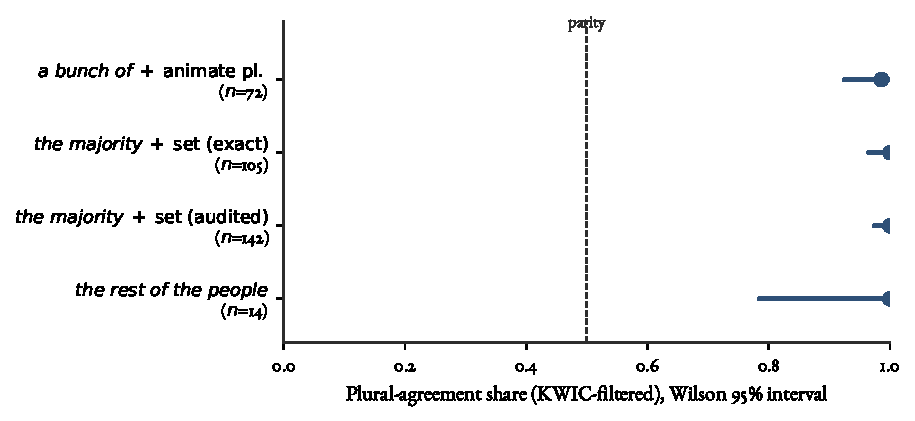
\includegraphics[width=0.82\textwidth]{fig_agr_projection.pdf}
\caption{Production-choice evidence for a prescriptively salient agreement
contrast. Plural-agreement share (dot) with Wilson 95\% interval (bar) for
collective-partitive subjects in \abbr{coca}, after \abbr{kwic} filtering to
subject-position tokens; the dashed line marks parity (no directional
preference). The share is a licensing indicator only conditional on independent
norming of candidate and outside-option choice. Data:
\texttt{agr-coca-projection} probe (\mention{bunch},
\mention{majority}/\mention{minority}, and partitive cells). Notional plural
dominates in each of the three constructional cells, and the interval widens
with the smaller denominators rather than drifting toward parity.}
\label{fig:agr-projection}
\end{figure}

Table~\ref{tab:agr-cells} makes the figure auditable: exact filtered cell counts, so the estimate can be checked rather than taken on trust.

\begin{table}[H]
\centering
\caption{Filtered agreement cells behind Figure~\ref{fig:agr-projection}. Counts are \abbr{kwic}-filtered subject-position tokens in \abbr{coca}; \enquote{pl.}\ and \enquote{sg.}\ are plural- and singular-agreement targets. The surface-head baseline predicts singular; the observed share is plural.}
\label{tab:agr-cells}
\begin{tabular}{@{}lrrrl@{}}
\toprule
Cell & pl. & sg. & $N$ & Plural share (Wilson 95\%)\\
\midrule
\mention{a bunch of} + animate pl. & \liningnums{71} & \liningnums{1} & \liningnums{72} & 0.986 (0.925--0.998)\\
\mention{the majority} + set (exact) & \liningnums{105} & \liningnums{0} & \liningnums{105} & 1.000 (0.965--1.000)\\
\mention{the majority} + set (audited) & \liningnums{142} & \liningnums{0} & \liningnums{142} & 1.000 (0.974--1.000)\\
\mention{the rest of the people} & \liningnums{14} & \liningnums{0} & \liningnums{14} & 1.000 (0.785--1.000)\\
\bottomrule
\end{tabular}
\end{table}

\subsection{Worked examples: deriving status from the posterior}
\label{sec:worked-examples}

The examples from \S\ref{M-sec:diag-tree} show how population status and its
posterior estimate are related.
The winnerless cell adds the case where concentration carries the phenomenology
rather than merely labelling it.

\begin{enumerate}
\item \ungram{\mention{Can the have running}} (nonsense).
  $\mathcal{A}(f,v)=\emptyset$: no covering assembly in the fixed inventory.
  $S_t^{\theta}=G_t=0$ up to inventory uncertainty; $\Phi\approx1$ under every
  construal. Status: ungrammatical, structurally.

\item \mention{Colorless green ideas sleep furiously}. A covering assembly is defined, saturated, and licensed node by node: $S_t^\theta\approx1$, with $G_t$ and a typical $g_{i,t}$ tracking it. The strangeness is a construal-plausibility cost in $R_i$: $F$ negative, status grammatical. Content-odd, not ill-formed.

\item \ungram{\mention{I've finished it yesterday}} (compatibility failure). Covering assemblies exist, but every one sets the reference-interval dimension twice incompatibly--the perfect's contribution and the deictic adverb's don't unify--so $\operatorname{def}(A)=0$ throughout. $S_t^{\theta}=G_t=0$; $\Phi\approx1$. Entrenchment of the component constructions can't repair it: the clash is outside the licensing terms altogether.

\item \ungram{\mention{I have 25 years}} (licensing failure). Defined and saturated; the intended value is recoverable. The pivotal age-predication node has $\theta_t\approx0$, tracked by a typical speaker at $C^{(i)}_t\approx0$ with high $\nu^{(i)}$, after preemption by the \textsc{be}-frame in a dense niche. $g_{i,t}\approx0$ and $\Phi$ is high. Status: ungrammatical, by concentrated non-licensing.

\item \marg{\mention{friend of whose}} (community-novel). Defined and saturated; the niche is vanishingly sparse, so a typical speaker's pivotal-node posterior sits near its prior with low $\nu^{(i)}$. The speaker's $g_{i,t}$ is intermediate, $\operatorname{Var}(S_t^{\theta}\mid\mathcal{D}_{i,t})$ is high, and $\Phi$ is low. Status: unsettled (starved); framing-movable, with surprisal adding $R$-channel noise.

\item \ungram{\mention{Which did you buy car?}} (putative preempted gap).
Defined and saturated; the dedicated discontinuity node--the only activated node
covering the determiner--head discontinuity--receives negative evidence from
fronting opportunities only in proportion to independently normed
$\widetilde{\rho}_t^\star$. If that full-choice term is high, its posterior is
driven to zero and concentrates there (\S\ref{sec:update}); if it's low, the
case belongs closer to starvation. Status assignment requires the niche-norming
protocol of \S\ref{sec:identification-c}.

\item \mention{pobedit'} \abbr{1sg} (winnerless cell; \ungram{\mention{amn't}} as a mixed case). The niche is dense and candidate assemblies have readily recoverable values, but candidate support is weak and no candidate accumulates positive evidence--the outside option absorbs production, and because avoidance has low attributability, candidates accumulate little confident negative evidence either (\S\ref{sec:winnerless-cells}). Given that low support, every candidate's pivotal node has a low speaker-level mean and low $\nu^{(i)}$. The typical $g_{i,t}$ is low, $\operatorname{Var}(S_t^{\theta}\mid\mathcal{D}_{i,t})$ is high, and $\Phi$ is low. Status: unsettled (avoidance-divided); phenomenology ineffability, not rejection--same mean as a preempted gap, different concentration, different feeling.

\item \mention{The bread the baker the apprentice helped made is delicious} (processing overload). A typical $g_{i,t}$ is high; the locality term in $R_i$ is large. $F$ is negative and $\Phi$ moderate; satiation and instruction move the $R$ contribution, not the licensing posterior. Status: grammatical, transiently ill-felt.
\end{enumerate}

Figure~\ref{fig:posterior-means} shows the low-opportunity versus dense-preemption contrast that underwrites several of these classifications.

\begin{figure}[t]
\centering
\begin{tikzpicture}
\begin{axis}[
    width=0.8\textwidth,
    height=7cm,
    xlabel={Experience (steps)},
    ylabel={Licensing posterior (mean, 95\% CrI)},
    xmin=0, xmax=50,
    ymin=0, ymax=1,
    grid=major,
    legend entries={Rare (sparse opportunities), Dense preemption},
    legend pos=north east
]
\addplot[name path=rarehi, draw=none, forget plot]
  table[x=step,y=sparse_hi] {simulation_data.dat};
\addplot[name path=rarelo, draw=none, forget plot]
  table[x=step,y=sparse_lo] {simulation_data.dat};
\addplot[blue, fill opacity=0.10, forget plot] fill between[of=rarehi and rarelo];
\addplot[name path=densehi, draw=none, forget plot]
  table[x=step,y=dense_hi] {simulation_data.dat};
\addplot[name path=denselo, draw=none, forget plot]
  table[x=step,y=dense_lo] {simulation_data.dat};
\addplot[red, fill opacity=0.10, forget plot] fill between[of=densehi and denselo];
\addplot[mark=none, blue, thick]
  table[x=step,y=sparse_mean] {simulation_data.dat};
\addplot[mark=none, red, thick, dashed]
  table[x=step,y=dense_mean] {simulation_data.dat};
\end{axis}
\end{tikzpicture}
\caption{Licensing posteriors under the affine omission likelihood, from a $\mathrm{Beta}(1,1)$ prior. The sparse arm receives one attributable omission every ten steps (five total); the dense arm receives a batch of five per step (250 total). Each omission has $d=.495$, derived from equal-utility candidates and outside utility $-4$. After each step, the exact finite mixture is projected to a Beta distribution by matching its first two moments. Lines show posterior means; shading gives 95\% Beta intervals. Sparse evidence leaves a broad posterior even as its mean moves, while dense preemption lowers the mean and raises concentration. The data is generated by \texttt{simulate\_dynamics.py}; population actuation also requires the transition in~\eqref{eq:inclusion-transition}.}
\label{fig:posterior-means}
\end{figure}


\section{Dynamics: candidate routes to stabilization}
\label{sec:dynamics}

The dynamics module explains trajectories of construction-level licensing
posteriors, and in principle refinements of the conditioning partition itself.
It doesn't define grammaticality.

\subsection{Niches, competitors, and opportunity sets}
\label{sec:niches}

Let $n$ index a \term{constructional niche} (a communicative job), and let
$\mathcal{V}_{n,t}^{\star}$ be the opportunity set: the attested,
hierarchically constructible, and analogically generated candidate realizations
that could plausibly do that job in some conditioning states. Membership in
this set doesn't presuppose that a candidate is licensed.
Let $N_t(n,c)$ be the number of opportunities for niche $n$ in conditioning
state $c$ during the current window $W_t$, and $k_t(x,n,c)$ the observed count of
candidate realization $x\in\mathcal{V}_{n,t}^{\star}$.

The star matters. Preempted gaps and innovations often involve candidates with no
positive tokens. Their counterfactual utilities are still defined because the
hierarchy $\mathcal{H}$ generates analogical candidates. English learners can
represent a left-branch extraction candidate by combining interrogative
fronting, modifier--noun packaging, and question formation, even if no one
licenses that candidate as an English resource. The same machinery lets a novel
but ordinary sentence inherit coverage from licensed higher-grain constructions
rather than being preempted merely because that exact sentence type is new.

\subsection{Usage as \texorpdfstring{licensing $\times$ choice}{licensing x choice} among candidates}
\label{sec:usage}

Separate \term{licensing} from \term{selection}. A candidate can be licensed but
rarely chosen.

Let $\rho_t^\star(x\mid n,c)\in[0,1]$ be the candidate-conditional
counterfactual probability of choosing $x$ if every registered candidate were
available in niche $n$ under $c$. A flexible choice model is a softmax over
utilities:
\[
\rho_t^\star(x\mid n,c)=
\frac{e^{U_t(x;n,c)}}{\sum_{x'\in\mathcal{V}_{n,t}^{\star}}e^{U_t(x';n,c)}},
\qquad
U_t(x;n,c)=\mathbf{w}^{\top}\mathbf{f}(x;n,c).
\]
Because the production model also contains an outside option, the quantity that
enters a licensing--usage factorization is instead the full-choice share
\[
\widetilde{\rho}_t^\star(x\mid n,c)=
\frac{e^{U_t(x;n,c)}}
{e^{U_t(\bot;n,c)}+
 \sum_{x'\in\mathcal{V}_{n,t}^{\star}}e^{U_t(x';n,c)}}.
\]
The two coincide only when the outside option has negligible mass. Empirical
norming has to offer the relevant avoidance, periphrasis, or
repair-in-progress response as well as the candidate realizations; a
candidate-only forced choice estimates $\rho_t^\star$, not
$\widetilde{\rho}_t^\star$.

At the population level, the expected usage rate is
\[
\pi_t(x\mid n,c)=
E_i\!\left[
\frac{z_i(x,c)e^{U_t(x;n,c)}}
{e^{U_t(\bot;n,c)}+
\sum_{x'\in\mathcal{V}_{n,t}^{\star}}z_i(x',c)e^{U_t(x';n,c)}}
\right],
\]
where, for a candidate $x$ with form--value pair $(f_x,v_x)$,
\[
z_i(x,c)=\mathbf{1}\!\left[
\exists A\in\mathcal{A}(f_x,v_x):
\operatorname{def}(A)\wedge\operatorname{sat}_t(A,c)\wedge
\bigwedge_{\kappa\in A}z_{i,t}(\kappa,c)
\right]
\]
abbreviates speaker $i$'s availability of a complete licensed route for $x$
(with the time index suppressed on the left), and $\bot$ is the outside option
(avoidance, periphrasis, or repair-in-progress). A candidate realization appears
once in the softmax: if several assemblies license the same realization, the
existential above aggregates them into the single gate $z_i(x,c)$ rather than
adding separate choice masses. With several required nodes,
the expectation is evaluated over the joint inclusion model rather than inferred
from marginal node means alone. When one pivotal availability gate dominates
and the other gates and full-set choice weights have been normed independently,
the predictive product
$\pi_t(x\mid n,c)\approx S_t^\theta(x,c)
\widetilde{\rho}_t^\star(x\mid n,c)$ is a useful population-level
approximation. In single-pivotal-node cases this reduces to
$\theta_t(\kappa_x,c)\widetilde{\rho}_t^\star(x\mid n,c)$, where $\kappa_x$ is
the node that would realize $x$ in $c$. The corresponding analyst prediction
replaces $S_t^\theta$ with $G_t$, or $\theta_t$ with $\widehat C_t$, as an
estimation step; it doesn't identify the ontic usage rate with the estimate.
The full-choice term can be high even when the population availability is near
zero, so absence becomes informative under that condition.

\subsection{Dynamics: evidence streams, weighted omissions, and repair}
\label{sec:update}

Speaker $i$ represents each construction--situation pair $(\kappa,c)$ with a
Beta filter over the population licensing rate $\theta_t(\kappa,c)$
(\S\ref{sec:objects}); the analyst may use the same family on a different data
stream. The Beta is exact after direct Bernoulli inclusion observations, but the
observable data here are gated choices. A target choice supplies a factor
proportional to $\theta$; a non-target choice supplies an affine factor in
$\theta$. The resulting finite-window posterior is generally a Beta mixture.
The bounded filter below projects that exact mixture back to Beta by matching
its first two moments.

Discount accumulated evidence before applying the new window. For baseline
prior $\mathrm{Beta}(a^0,b^0)$ and memory $\delta_m\in(0,1]$, put
\begin{equation}
\widetilde a_t=a^0+\delta_m(a_t-a^0),\qquad
\widetilde b_t=b^0+\delta_m(b_t-b^0).
\label{eq:baseline-discount}
\end{equation}
A quiet filter returns to its stated prior. The recurrence discounts the
accumulated state, and the current window enters once. Setting $\delta_m=1$
gives a fixed-parameter filter, while $\delta_m<1$ is an assumed-density dynamic
filter for a drifting convention \citep{WestHarrison1997}.

Consider a non-target outcome $y_j\ne x$. Let
\begin{equation}
\ell_j(x)=\log P(y_j\mid Z_x=0,n,c)-
\log P(y_j\mid Z_x=1,n,c)
\label{eq:attributability}
\end{equation}
be its omission log likelihood ratio, used here as an information diagnostic.
The update itself uses the probability-space contrast below. With $r_j\in[0,1]$
the independently coded probability that the occasion is attributable to the
target niche, define
\begin{equation}
d_j=r_j\left(1-
\frac{P(y_j\mid Z_x=1,n,c)}{P(y_j\mid Z_x=0,n,c)}\right)\in[0,1].
\label{eq:preemption-mass}
\end{equation}
Marginalizing the latent availability state
$Z_x\sim\mathrm{Bernoulli}(\theta)$ gives, up to a constant independent of
$\theta$,
\[
P(y_j\mid\theta,n,c)\ \propto\ 1-d_j\theta.
\]
Attribution scales $d_j$ in probability space: with probability $1-r_j$ the
event is uninformative, and with probability $r_j$ it carries the full
counterfactual contrast.

If the window contains $s_t$ target choices and $m_t$ non-target choices, its
exact posterior kernel after~\eqref{eq:baseline-discount} is
\begin{equation}
p_{t+1}(\theta)\ \propto\
\theta^{\widetilde a_t-1+s_t}(1-\theta)^{\widetilde b_t-1}
\prod_{j=1}^{m_t}(1-d_j\theta).
\label{eq:affine-window-posterior}
\end{equation}
The affine product has the Bernstein expansion
\[
\prod_{j=1}^{m_t}(1-d_j\theta)=
\sum_{k=0}^{m_t}c_k\theta^k(1-\theta)^{m_t-k},
\]
where $c^{(0)}_0=1$ and
$c^{(j+1)}_k=c^{(j)}_k+(1-d_{j+1})c^{(j)}_{k-1}$, with out-of-range
coefficients zero. Hence~\eqref{eq:affine-window-posterior} is exactly a mixture
of at most $m_t+1$ Betas,
\[
\mathrm{Beta}(\widetilde a_t+s_t+k,
              \widetilde b_t+m_t-k),
\]
with normalized weights proportional to the corresponding $c_k$ times the
Beta normalizer. Let $\mu_{t+1}$ and $v_{t+1}$ be that mixture's exact mean and
variance. The bounded assumed-density step is
\begin{align}
\nu_{t+1}&=\frac{\mu_{t+1}(1-\mu_{t+1})}{v_{t+1}}-1, &
a_{t+1}&=\mu_{t+1}\nu_{t+1}, &
b_{t+1}&=(1-\mu_{t+1})\nu_{t+1},\\
C_{t+1}&=\frac{a_{t+1}}{a_{t+1}+b_{t+1}}.
\label{eq:beta-update}
\end{align}
This projection preserves the exact first two posterior moments but not, in
general, higher moments. Its approximation error is part of the model
audit. Direct target observations, $d_j=0$, and $d_j=1$ recover the relevant
conjugate limits.

The equations describe one pivotal availability gate. If a token's parse or
niche attribution is uncertain, that uncertainty is marginalized in its
likelihood before $d_j$ is calculated. A multi-node target requires
the joint inclusion model from \S\ref{sec:objects}; one omission LLR can't be
split into independent node failure counts.

Population change enters through an explicit learner-to-population transition
kernel. Let $C^{(i)}_{\kappa,c,t}$ and $\nu^{(i)}_{\kappa,c,t}$ be speaker $i$'s
filter summaries, let $\xi_{i,t}$ collect lect, network, and other independently
specified adoption covariates, and let $\lambda_{i,\kappa}\in[0,1]$ govern
persistence. Then
\begin{equation}
z_{i,t+1}(\kappa,c)\sim\operatorname{Bernoulli}\!\left(
  (1-\lambda_{i,\kappa})z_{i,t}(\kappa,c)+
  \lambda_{i,\kappa}h_\kappa(C^{(i)}_{\kappa,c,t},
    \nu^{(i)}_{\kappa,c,t},\xi_{i,t},c)\right),
\label{eq:inclusion-transition}
\end{equation}
where $h_\kappa\in[0,1]$ is an adoption--retention response fixed independently
of the outcome being predicted. The numerical analysis below uses
\begin{equation}
h_\kappa(C,\nu;q_\kappa)=
P(\theta\geq q_\kappa\mid C,\nu),
\label{eq:posterior-threshold-adoption}
\end{equation}
which can be read as posterior sampling against an adoption criterion.
$q_\kappa$ has to be fixed from independently measured switching or coordination
costs, while concentration supplies the response's curvature. This causal
transition parameter is distinct from the judge's non-constitutive read-out
threshold $\tau(c)$ in \S\ref{sec:decision-readout}. A logistic
response to $C-q_\kappa$ remains a reduced-form sensitivity analysis only when
its slope is independently estimated. The persistence term allows stable individual
lects even when the population is divided. For a finite population of $M$
speakers, distinguish the empirical prevalence
\[
\theta^{(M)}_{t+1}(\kappa,c)=\frac{1}{M}\sum_{i=1}^{M}
z_{i,t+1}(\kappa,c)
\]
from the exchangeable rate $\theta_{t+1}$. Conditional on the current population
state, the expected empirical prevalence is the average of the transition
probabilities in~\eqref{eq:inclusion-transition}; in a homogeneous mean-field
case the realized prevalence fluctuates around that common probability at
$O_p(M^{-1/2})$. Replacing the average of a nonlinear $h_\kappa$ by its value at
average covariates is a separate closure approximation whose error depends on
population heterogeneity, not on the opportunity count $N_t$. Speakers'
evidence states can mediate population change, while an analyst's
posterior remains only a measurement of that change.
\noindent\textsc{Counterfactual informativeness.} When $y_i$ is an
in-repertoire competitor, let
\[
D_{0,i}=e^{U_t(\bot;n,c)}+
  \sum_{x'\ne x}z_i(x',c)e^{U_t(x';n,c)}
\]
be the gated normalizer when $x$ is unavailable, and define the occasion-level
full-choice share
\[
\widetilde{\rho}_{i,t}^\star(x\mid n,c)=
  \frac{e^{U_t(x;n,c)}}{D_{0,i}+e^{U_t(x;n,c)}}.
\]
Holding the other gates fixed, normalized softmax choice then gives the exact
identity
\[
\frac{P(y_i\mid Z_x=1,n,c)}{P(y_i\mid Z_x=0,n,c)}
  =1-\widetilde{\rho}_{i,t}^\star(x\mid n,c),
\]
and hence
\[
\ell^{\mathrm{omit}}_{i,t}(x)
=-\log\!\bigl(1-\widetilde{\rho}_{i,t}^\star(x\mid n,c)\bigr)
  \approx \widetilde{\rho}_{i,t}^\star(x\mid n,c)
\]
only when the target's full gated mass is small. The common
$N_t\cdot\rho_t^\star$ score is recovered as a small-mass information
approximation in a near-complete gap and
under four further conditions: nearly every opportunity is an attributable
omission ($r_i\approx1$), the outside option has negligible mass, the other
candidate gates match the norming task, and the target mass is small enough for
the log expansion. Continued attributable competitor choices can keep
supplying evidence against a concentrated gap; reopening it requires an
actuation route that changes utilities, gates, or the observed likelihood.

When $y_i$ is the outside option--periphrasis or avoidance, available at fixed
utility under both hypotheses--the same denominator identity applies. Its
choice is nearly uninformative only when the target's full counterfactual mass
$\widetilde{\rho}_{i,t}^\star$ is small, which requires $x$'s utility to be low
relative to the candidate set and the outside option. That condition is
independently estimable from the same norming task. Then
$\ell^{\mathrm{omit}}_{i,t}(x)\approx0$.

When candidate support is weak, the affine contrast lets periphrasis remain
weak evidence against any one candidate. This separates the defective cell's
low-concentration state from the preempted gap's high-concentration state
(\S\ref{sec:winnerless-cells},
\S\ref{sec:worked-examples}).

\noindent\textsc{The repair stream: a candidate controller.}
\label{sec:repair-controller}
The paper's support claims come in grades: stabilization, maintenance, control
(\S\ref{M-sec:implications}). The transition and full map below specify
candidate conditions for stabilization; showing that it or the proposed loop
supports an actual linguistic profile requires longitudinal or intervention
evidence. Control needs the stronger result that a process registers departures
from the licensed profile and pushes the population back. Conversational repair
is the candidate considered here.

Let $\Delta(d)$ be the expected common-ground divergence from mis-setting
operator dimension $d$: the quantitative face of \enquote{update-configuring}
in the working test of \S\ref{M-sec:operator-values}. Formally, $\Delta(d)$ is an
expected KL divergence between the common-ground posterior induced by the
intended value and the posterior induced by the mis-set value, in the same
spirit as RSA-style update models \citep{GoodmanFrank2016}. When a token
mis-sets $d$, update-oriented repair occurs with probability
$r_{\mathrm{upd}}(\Delta,\iota)$, increasing in $\Delta$ and modulated by
footing $\iota$. A different stream targets a value-intact exponent or
construction whose licensing evidence has concentration $\nu$; write its
probability as $r_{\mathrm{form}}(\nu,\iota)$. Over a window with
$N_t(n,c)$ opportunities, the two candidate repair exposures are
\begin{equation}
\begin{aligned}
\psi_{\mathrm{upd}}(n)
  &=N_t(n,c)\,P(\text{wrong value})\,
    r_{\mathrm{upd}}(\Delta,\iota),\\
\psi_{\mathrm{form}}(n)
  &=N_t(n,c)\,P(\text{value intact, form excluded})\,
    r_{\mathrm{form}}(\nu,\iota).
\end{aligned}
\label{eq:repair-flow}
\end{equation}
The first magnitude increases with divergence through $r_{\mathrm{upd}}$; the
second can remain high when $\Delta\approx0$ because the intended update is
intact while the form is strongly excluded. These are candidate repair
exposures, not yet derived terms in the likelihood-consistent filter.

The numerical results in \S\ref{sec:emergent-categoricality} supply no evidence
for the repair hypothesis; the companion software's programmed repair
comparison is only a diagnostic. Repair earns controller status under
Woodward's interventionist criterion if an
intervention on it changes the profile's return-to-attractor behaviour in an
invariant, predictable way \citep{woodward2001,
woodward2003MakingThingsHappen}. Until then, repair remains a testable candidate
controller.

Two commitments follow. First, the account predicts a distribution over repair
targets, not a binary grammar/style split. Opportunity is estimable from
opportunity-annotated corpora; $\Delta$ comes from comprehension probes fixed
before the repair data is inspected; and $\nu$ comes from the independent
licensing evidence. A closed, dense contrast with $\Delta\approx0$ may still be
categorically excluded through constructional or exponent licensing, and may
attract form correction. What it should lack is the update-oriented
repair profile predicted by $r_{\mathrm{upd}}$. Second, if that repair profile
tracks social indexing rather than $\Delta$ after the other factors are held
fixed, the proposed operator-directed controller fails cleanly. Blythe and
Croft's utterance-selection dynamics remain the no-repair special case, so the
import is conservative \autocite{BlytheCroft2012}.

\noindent\textsc{Grain asymmetry and compositional inheritance.} Positive and
negative evidence can bear on different constructional grains. A heard token
supports the activated constructions that sanction its observed properties.
An attributable omission instead bears on the complete candidate-level route
that would have made the missing realization available. In Bayesian terms, the
likelihood penalty for structured non-occurrence falls on a hypothesis that
wastes choice probability on unobserved sentence types
\autocite{PerforsEtAl2011}.

Compositional inheritance raises an objection. Token-level licensing is assembled from
constructional nodes, so left-branch extraction activates the well-licensed
nodes for interrogative fronting, question formation, and modifier--noun
packaging. Their independent support might then seem to make the discontinuous
candidate available.

That result doesn't follow from the status definition. Availability requires a
complete licensed route, and those parent nodes sanction only \emph{contiguous}
realizations. None of them covers the
determiner--head discontinuity that defines
\ungram{\mention{Which did you buy car?}}; producing that token requires a node
that licenses a determiner--head arc crossing the verb, and no
contiguity-preserving node in $\mathcal{H}$ generates one
\autocite{reynolds2026lbe}.

The parents can retain high licensing on the strength of their abundant
contiguous tokens without licensing the discontinuous route. If the grammar
posits a dedicated left-branch-extraction node, its licensing has to be
estimated separately. Attributable omissions then bear on the candidate-level
gate only to the extent that competitors would have been chosen instead, which
is why the independent $\widetilde{\rho}_t^\star$ norming required in
\S\ref{sec:identification-c} is necessary.
This asymmetry also answers an acquisition worry. If token-level licensing were
just pooled parent licensing, learners should pass through a stage of treating
left-branch extraction as live. They don't need to: the candidate is generated
by analogy, so it's on the table with non-zero prior support, but its dedicated
node has no scaffolding of its own, fronting opportunities are dense in the
input, and each one adds preemption mass.

The quantitative model in this supplement updates a candidate-level pivotal
gate. It doesn't yet define fractional evidence allocation across all activated
nodes or a numerical pooling rule. Evidence distribution through a construction
hierarchy remains a further modelling problem; the equations here don't settle it.

A companion corpus study quantifies
one side of the evidential situation: across 1{,}228 fronting opportunities in a
sixteen-corpus Universal Dependencies sample, zero genuine determiner--head
discontinuities occur (95\% upper bound 0.24\%), while contiguity-preserving
alternatives (pied-piping, fused-head construals, and the \mention{big mess}
family) occur at measurable rates \autocite{reynolds2026lbe}. Comprehension
pushes the same way: a fronted \mention{whose} or \mention{which} defaults to a
fused-head parse, so the discontinuous analysis also loses the parsing race
\autocite{Culicover_Varaschin_Winkler_2022_Radical}. What remains to be normed
is $\widetilde{\rho}_t^\star$: if speakers would rarely choose the discontinuous form even
under a permissive stipulation that English allowed it, the absence would support
starvation rather than preemption. The predicted non-satiation of left-branch
extraction remains a test; \posscite{Lu2024} meta-analysis of
satiation in extraction from islands supplies the closest current analogue, not
a direct measurement of \abbr{lbe} itself.

\noindent\textsc{Open-loop learning and closed-loop dynamics.} The discrete
update~\eqref{eq:beta-update} changes an evidence state in a fixed exogenous
environment. Figure~\ref{fig:posterior-means} shows the resulting evidential
difference between sparse and dense attributable omissions. Population
bifurcation requires the transition in~\eqref{eq:inclusion-transition}:
inclusion gates production, production supplies later choice evidence, and
speaker filters affect later adoption and retention.

\subsection{Conditional emergence of separated regimes}
\label{sec:emergent-categoricality}

The sense of \term{emergence} used here is weak and mechanistic:
population-level categoricality is a possible outcome of learner updating,
adoption, and selection. This differs from Hopper's \enquote{emergent grammar}, where grammar is
perpetually provisional \autocite{hopper1987}.

For a homogeneous focal candidate, let
$X_t=(\theta_t,a_t,b_t)$ and let
$\mathcal M_{\theta_t}(a_t,b_t)=(a'_t,b'_t)$ be the deterministic
expected-window version of the discounted likelihood update in
\eqref{eq:affine-window-posterior}. It uses the expected target and non-target
counts implied by the gated-choice model and moment-matches the resulting
power-likelihood posterior. The composed mean-field map is
\begin{equation}
F(X_t)=\left(
(1-\lambda)\theta_t+\lambda h_\kappa(a'_t,b'_t),
a'_t,b'_t\right).
\label{eq:full-mean-field-map}
\end{equation}
This expected-window closure is a deterministic diagnostic of the
finite-population stochastic process, whose transition kernel remains
\eqref{eq:inclusion-transition}. Fixed points satisfy
$F(X^\ast)=X^\ast$; their local stability is governed by the full Jacobian,
\begin{equation}
\rho\!\left(J_F(X^\ast)\right)<1,
\label{eq:full-map-stability}
\end{equation}
where $\rho$ is spectral radius. This criterion retains the slow evidence
directions that a scalar population equation discards.

A reduced crossing plot remains useful for location. Let $\eta$ be expected
opportunity inflow per step before observation and let $q$ be the adoption
threshold. Holding $\theta$ fixed, let
$(a^\ast_{\eta}(\theta),b^\ast_{\eta}(\theta))$ be the stationary evidence state
and put
\[
H_{\eta,q}(\theta)=
h_{\kappa,q}(a^\ast_{\eta}(\theta),b^\ast_{\eta}(\theta)),
\qquad
R(\theta;\eta,q)=H_{\eta,q}(\theta)-\theta.
\]
Here $h_{\kappa,q}(a,b)$ abbreviates
$h_\kappa(a/(a+b),a+b;q)$ from
\eqref{eq:posterior-threshold-adoption}.
Zeros of $R$ locate candidate equilibria. They do
not supply return times: the scalar derivative can differ sharply from the
dominant eigenvalue of~\eqref{eq:full-map-stability} when evidence is slow.
The unstable interior crossing is denoted $\theta^\ddagger$ below.

The numerical analysis uses a specified two-candidate cell: equal candidate
utilities, outside utility $-4$, twelve opportunities per step, observation
probability $.6$, memory $.96$, inclusion-update rate $.08$, a uniform Beta
baseline, and $q_\kappa=.5$. Under the posterior-threshold response in
\eqref{eq:posterior-threshold-adoption}, the deterministic closure has stable
fixed points effectively at $0$ and $1$ and an unstable crossing at
$\theta^\ddagger\approx .493$. The corresponding spectral radii are $.961$,
$1.087$, and $.971$. A logistic reduced form with slope $8$ has stable fixed
points near $.024$ and $.968$ around an unstable crossing near $.489$; slope
$4$ has only one stable interior fixed point. A proportional response likewise
has one interior fixed point. Thus the independently specified adoption response
supplies the nonlinearity.

Finite-population runs preserve that scope result. Across 36 seeded runs of 320
steps initialized at $.1$, $.5$, and $.9$, the posterior-threshold and
slope-$8$ responses both passed the declared basin-separation and endpoint
criteria; the proportional response didn't. A dominant outside option
($U(\bot)=5$) produced weak evidence and no endpoint concentration. Moderate
inclusion-only and evidence-state perturbations returned to both attracting
regions. These runs establish existence and scope for the declared process.
They provide neither an empirical fit nor a stationary-distribution result. The
exact grid, seeds, approximation diagnostics, and artifact hash are archived
with the companion software.

\noindent\textsc{Local bifurcation diagnostic.} The full expected-window closure
has a codimension-two cusp of fixed points if
\begin{equation}
R=\partial_\theta R=\partial^2_\theta R=0,
\qquad
\partial^3_\theta R\neq0,
\qquad
\det
\begin{pmatrix}
\partial_\eta R & \partial_q R \\
\partial_{\theta\eta}R & \partial_{\theta q}R
\end{pmatrix}
\neq0,
\label{eq:cusp-conditions}
\end{equation}
provided the full map has one unit eigenvalue and stable transverse
eigenvalues. These are local fixed-point conditions; they neither introduce a
potential nor invoke a global catastrophe classification.

Numerical continuation under the utilities, observation probability, memory,
and inclusion-update rate specified above, while varying $\eta$ and $q$, locates
the point
\[
(\theta_c,\eta_c,q_c)=(.370957,.479156,.552048),
\qquad
(a_c,b_c)=(1.798418,2.039839).
\]
The effective observed inflow is $.287494$. At the reported differentiation
scale, the first two state derivatives of $R$ are below $3\times10^{-8}$ in
absolute value, $\partial^3_\theta R=-7.2843$, and the unfolding determinant
is $2.3345$. The full-map eigenvalues are $1.000000031$, $.961496$, and
$.883699$; step-size audits preserve the non-zero third derivative and
determinant.

A nearby point inside the cusp wedge has fixed points at
$\theta\approx.253,.370,.505$, with stable outer points and an unstable middle
point; a point outside has one stable fixed point near $.230$. Five stationary
evidence solves from distinct initial states agree to within $10^{-8}$.

A quasi-static two-control cycle also distinguishes this geometry from a steep
single-valued response. Holding one local control coordinate fixed and sweeping
the other produces two static folds, at local biases $-.001041$ and $.000901$.
As the dwell time at each control value rises from 1{,}000 to 10{,}000 map
iterations, the directional jumps converge toward those folds.

The same current external controls can support different stable licensing
states when the retained evidence state differs. An empirical application would
have to estimate effective exposure and the adoption threshold without fitting
them to the transition points being explained.

\noindent\textsc{Slowing and its failed stochastic proxy.} At $q=.5$, the
lower-branch fold occurs at $\eta=.654741$. As the deterministic state approaches
that fold from $2.5$ to $1.02$ times the fold inflow, the dominant spectral
radius rises from $.964802$ to $.995641$, its implied relaxation time rises from
28 to 229 windows, and measured pulse recovery rises from 82 to 288 windows.
This establishes deterministic slowing in the expected closure.

It doesn't establish a usable stochastic early-warning signal. In the
finite-population diagnostic, each of four fold distances had 24 runs with 240
speakers over 3{,}000 steps. Median detrended variance and lag-one
autocorrelation rose through the $1.1$ condition, but 23 of 24 paths escaped
there. At $1.02$, all paths escaped, only four supplied a usable pre-escape
segment, and both summaries fell. The preregistered monotonicity and
minimum-replicate gates fail.

That diagnostic also uses one opportunity per step with observation probability
set to effective inflow; other opportunity--observation factorizations remain
untested. The local
bifurcation and deterministic hysteresis survive this failure, but no general
observable early-warning prediction follows.

The convergence claim has to match both levels of the model. With perfect
retention ($\delta_m=1$), an individual evidence filter is close to
reinforcement processes of Pólya type, where stochastic approximation supplies
relevant techniques \citep{pemantle2007}. The signaling-game case,
structurally the closest analogue, is treated directly by Argiento, Pemantle,
Skyrms, and Volkov \citep{argiento2009}, with an extension by Hu, Skyrms,
and Tarrès \citep{huSkyrmsTarres2011}. Those results don't establish
convergence of the composed population transition
in~\eqref{eq:inclusion-transition}; that requires a specified $h_\kappa$.

With bounded memory ($\delta_m<1$), the learner filters have constant gain, so
the decreasing-gain analogues no longer prove almost-sure convergence even at
that level. The population-level formal target is a stationary distribution for
the composed transition concentrated near the full map's attracting regions,
with escape times and residual dispersion set by opportunity, persistence, and
memory: high-opportunity contrasts should sit tightly near the extremes, while
low-opportunity or outside-option-dominated contrasts remain diffuse. That claim is a proof
obligation rather than a theorem here.

The operator-specific prediction also needs its scope stated. Neither the full
map nor the local bifurcation diagnostic derives the operator-specific response
boundary. The OVMG claim is
conditional: adoption criteria and selection intensity have to vary with
independently estimated switching or coordination costs, opportunity, and
update divergence. Under that condition, dense, update-configuring contrasts
may concentrate faster.

Low $\Delta$ doesn't by itself imply gradient
licensing: a construction or exponent can be categorically excluded by dense
competitor evidence without being an operator. The operator-specific claim is
instead about comprehension and repair type. If a closed, dense,
non-configuring contrast shows the same update-confusion and update-oriented
repair profile as a matched operator contrast, that part of the account fails.

Bounded memory adds a quantitative residual: even near an attractor, dispersion
should scale with opportunity and forgetting, roughly with the effective
concentration supplied by the discounted evidence filter.

Sampling drift near the extremes makes the boundaries sticky in finite
populations, while middle states stay vulnerable to renewed evidence. The same
escape-time logic connects winnerless-cell metastability (\S\ref{sec:winnerless-cells})
and actuation (\S\ref{sec:actuation}): a state can persist for long periods and
then move quickly once the observation likelihood or outside-option utility changes.
This connects the dynamics to complex-adaptive and cultural-evolutionary
accounts of language change \autocite{beckner2009,kirby2014,BlytheCroft2012},
and to invisible-hand explanations, where macro-level order emerges as the
unintended consequence of micro-level choices \autocite{keller1994}.

\subsection{Derived obligatoriness}
\label{sec:derived-obligatoriness}

The state theory defines saturation relative to the obligatory dimensions
$\mathrm{OBL}_t(n,c,A)$ (\S\ref{sec:objects}), where $n=n(A,c)$ is the
registered at-issue niche. Those dimensions are path-dependent population
properties, estimated separately by an analyst. Let
$\mathcal{A}_0(d,n,\phi,c)$ be the finite, independently fixed class of defined
assemblies of frame type $\phi$ that realize niche $n$ while leaving $d$ unset.
For $A$ in that class, define the population's \term{raw zero-marking rate}
\[
R_s^0(A,n,c)=P_j\!\left(\text{speaker $j$ realizes a $d$-at-issue opportunity
in $(n,c)$ with $A$ at $s$}\right).
\]
This realized population statistic is distinct from the licensing predicate
$L_s$ and from a status estimate. The same simple-present nodes can have high
licensing in a habitual niche while their zero-marked realization rate is near
zero in an ongoing-at-issue niche. General node availability, niche-specific
zero marking, and saturation remain separate quantities.

Let $W_t=[t-W,t)$ be a preceding convention-individuating window, and let
$\Pi_{W_t}(A,d,n,c)$ be the realized pressure against $A$ there: $d$-at-issue
opportunities in which a marked competitor wins, weighted by the independently
normed full-choice share $\widetilde\rho^\star$. This weight is ungated; it
doesn't use $\operatorname{sat}_s$ or $\mathrm{OBL}_s$. Outside-option choices
don't contribute. Write $E_t(d,n,\phi,c)$ for the entry condition that, for
every $A\in\mathcal A_0(d,n,\phi,c)$,
\[
\sup_{s\in W_t}R_s^0(A,n,c)<\epsilon_0
\qquad\text{and}\qquad
\Pi_{W_t}(A,d,n,c)\geq\pi_0.
\]
Write $X_t(d,n,\phi,c)$ for the release condition that, for some such $A$,
\[
\inf_{s\in W_t}R_s^0(A,n,c)>\epsilon_1
\qquad\text{or}\qquad
\Pi_{W_t}(A,d,n,c)\leq\pi_1,
\]
where $\epsilon_1>\epsilon_0$ and $\pi_1<\pi_0$. Given an initial convention
state $\mathrm{OBL}_{t_0}$ fixed independently of the target interval, the
path-dependent macro is
\[
d\in\mathrm{OBL}_t(n,c,\phi)
\quad\Longleftrightarrow\quad
E_t(d,n,\phi,c)\ \lor\
\bigl[d\in\mathrm{OBL}_{t-1}(n,c,\phi)\land
\neg X_t(d,n,\phi,c)\bigr].
\]

The entry clauses say that every zero-marking realization has persistently
disappeared under dense, attributable competition rather than because the niche
was starved or an outside option absorbed a winnerless cell. The release clauses
require sustained recovery or a clear pressure lapse. The two pairs of
thresholds leave a hysteresis band in which the preceding state persists. The
timescale and thresholds are
community-indexed model parameters fixed independently of the contrast being
classified. The initial condition and strict temporal descent make the
recursion well founded: realized outputs and ungated pressure in $W_t$, together
with $\mathrm{OBL}_{t-1}$, determine $\mathrm{OBL}_t$;
$\mathrm{OBL}_t$ determines $\operatorname{sat}_t$; and saturation then enters
$S_t^\theta$. This makes status a functional of the recent population
history, not just of instantaneous $\boldsymbol{\theta}_t$.

An analyst identifies $d$ as obligatory when the posterior upper bound for every relevant
$R_s^0(A,n,c)$ lies below $\epsilon_0$, the estimated pressure clears $\pi_0$, and the
effective evidence meets a preregistered $\nu_{\min}$. Those conditions warrant
an inference about the population property $\mathrm{OBL}_t$. Identification of
release analogously requires posterior evidence for $X_t$ across the registered
window.

The proposed mechanism is the population transition plus preemption applied to
zero-marking. In a $d$-at-issue niche, marked and unmarked assemblies compete;
where the marked assembly repeatedly wins, speakers' filters and later inclusion
states can drive the raw zero-marking rate down. The full map shows one
possible phase portrait for that process, while the stationary-distribution
claim remains a proof obligation rather than part of the definition of
obligatoriness.

The typological payoff is that \S\ref{M-sec:community-values}'s descriptions
convert to predictions. On the proposed diagnosis, English progressive marking
is obligatory because simple-present assemblies in ongoing-at-issue niches have
persistently low raw zero-marking rates under a winning marked competitor; French
zero-marking there hasn't, so the dimension stays optional, and
\mention{Elle étudie maintenant} is fine. Turkish evidential marking is the
same kind of hypothesis on a different dimension. Grammaticalization's
obligatorification receives a candidate mechanism: a contrast on its way
to obligatory status is one whose zero-marking competitor is losing dense
niches one at a time, which predicts an intermediate stage--obligatory in some
frame types and niches, optional in others--that grammaticalization corpora are
positioned to test.

\subsection{Winnerless cells}
\label{sec:winnerless-cells}

Preempted gaps have a winning competitor. Defective paradigm cells don't, and
the dynamics explain how the difference can be stable rather than transitional.

Suppose candidates $f_1,\dots,f_m$ for a dense cell have weak analogical support,
the outside option (periphrasis, avoidance) has moderate fixed utility, and
producing a weakly licensed form carries a face cost. Then the production rule
routes the cell's opportunities to the outside option: no candidate accumulates
positive evidence. The omission likelihood matters here: outside-option choices
have $\ell^{\mathrm{omit}}_{i,t}(x)\approx0$, so no candidate accumulates much negative evidence
either. Evidence starvation alone preserves the prior. The
low-mean/low-concentration profile requires an
additional independently motivated ingredient--low priors for unsupported
analogical candidates, weak diffuse negative evidence, a hierarchical prior over
defective cells, or a latent cell-level state such as \enquote{no candidate is
established}. Given such an ingredient, avoidance keeps every candidate at low
mean and low concentration, because escaping the state requires some candidate
to accumulate positive evidence that the outside option keeps starving it of.

The claim has two strengths. The winnerless-cell example in
\S\ref{sec:worked-examples} relies on the qualitative mechanism: an avoidance
attractor plus evidence starvation, with low prior support or weak diffuse
negative evidence supplying the low mean. The stronger metastability claim,
persistence for times exponential in population size, remains a conjecture with
analogues in evolutionary dynamics.
\posscite{Sims2023Defectiveness} point that the maintenance mixture varies
across cases--structural uncertainty, lexical restriction, learning dynamics,
avoidance--is compatible with this narrower claim: the model supplies the
avoidance-and-starvation component and is agnostic about the rest of the
mixture.

The phenomenological contrast is represented by the resulting evidence profile.
Clean defective cells
(\mention{pobedit'} \abbr{1sg}, with \ungram{\mention{amn't}} depending on niche
granularity) show low mean with
low concentration--\enquote{I don't know how to say it}--where preempted gaps
show low mean with high concentration--\enquote{that's impossible}. Same mean,
different concentration, different feeling, read out by $\Phi$
(\S\ref{sec:feeling-new}). The satiation-framing prediction follows: defective
cells should behave like low-evidence forms, movable under framing; preempted
gaps shouldn't \autocite{Broadbent2009Amnt,Pertsova2016RussianGaps,
ThomsEtAl2025Amnt}.

\subsection{Destabilization of moribund contrasts}
\label{sec:destabilization}

Bounded memory yields one more result. With discount $\delta_m<1$, the
equilibrium concentration of a node's posterior is set by the balance of
evidence inflow against forgetting:
$\nu^{\ast}\approx\nu_0+O\bigl(N_t(n,c)/(1-\delta_m)\bigr)$, with $N_t(n,c)$ the
per-window opportunity count for the node's niche and $\nu_0=a^0+b^0$ the baseline
concentration. If opportunity falls--a case distinction going moribund, a niche
drying up--equilibrium concentration falls toward the baseline. With no further
evidence, means drift toward the baseline prior under~\eqref{eq:beta-update};
with sparse, idiosyncratic evidence, individual histories can diverge. Falling
excess concentration is the direct consequence and the primary preregistrable
precursor; increasing test--retest instability is a behavioral proxy only if it
is independently validated against concentration.

Prior heterogeneity alone doesn't make dispersion lead the mean. If, after a
shared evidence stream disappears,
\[
C_{i,t}=w_t m_i+(1-w_t)C_E,
\]
where $m_i$ is speaker $i$'s baseline-prior mean, $C_E$ is the former common
evidence mean, and $w_t$ rises toward one, movement of the population mean is
linear in $w_t$ while between-speaker variance is
$w_t^2\operatorname{Var}(m_i)$. On a common fraction-of-eventual-change scale,
dispersion lags. The companion simulation reproduces this ordering at
both 25\% and 50\% progress. Dispersion-leading decline remains a conditional
hypothesis requiring a faster heterogeneity source, such as cohort replacement,
unequal network opportunity loss, heterogeneous retention, or a specified
judgment mapping.

\subsection{Actuation}
\label{sec:actuation}

In a bistable cell of the full map, \term{actuation} is movement of the coupled
population-and-evidence state across the basin boundary whose population
coordinate is $\theta^\ddagger$. A utility change, new target evidence, altered
outside-option mass, or a social change in $q_\kappa$ can move the state across
that boundary. Speakers' filters then alter adoption and retention through
\eqref{eq:inclusion-transition}. An analyst posterior should track the
population movement with a lag; motion in its mean isn't itself actuation.
No S-shaped time course follows without specifying the full perturbation and
the slow evidence state.

The factors that drive such bifurcations align with the motivations discussed
in \S\ref{M-sec:motivations}. Semantic reanalysis may increase utility (and thus
$\widetilde{\rho}_t^\star$) by making a form--value relation easier to interpret or more useful.
Social pressures may shift utilities (prestige effects) or alter the relevant
community standard. Structural motivations such as analogical extension can
systematically raise licensing probability by borrowing strength from frequent
neighbors. Processing innovations may reduce error rates or locality
costs, changing either the observation likelihood or later adoption.

Individual innovation is insufficient. A few speakers adopting a marginal
construction don't guarantee its success; the likelihood and transition have to
shift so that inclusion is systematically favoured across the relevant
community. Many sensible innovations fail because they appear before those
community conditions are in place.

Near the separatrix, small perturbations in community attitudes can trigger
rapid shifts between exclusion and licensing. As the state moves further past
$\theta^\ddagger$, reversal becomes increasingly unlikely. The full map can
represent the S-curves documented in some language changes
\autocite{kroch1989}. For constructions in the marginal zone, with the
population state near $\theta^\ddagger$, the model predicts
heightened sensitivity to external factors and greater cross-community
variation. Small or peripheral communities may show volatile behaviour near
bifurcation points before a change spreads to larger population centres.

The destabilization result sharpens the actuation picture at the other end of a
form's life. Actuation is crossing a separatrix; destabilization is a collapse
in concentration. A contrast can lose its grip when evidence of any kind stops
arriving, without accumulating negative evidence; the model predicts the two
routes are empirically
distinguishable: actuation crosses a basin boundary in the coupled state;
moribundity first removes evidence confidence and need not cross that boundary
until later population turnover. Judgment dispersion may lead only under the
additional heterogeneity mechanisms named above.

\subsection{Apparent exclusions from concentrated non-licensing}
\label{sec:categorical-without-bans}

When a defined, saturated assembly exists but its pivotal node's licensing
posterior is driven toward zero and concentrates there under persistent
preemption in a niche with many observed opportunities, speakers converge on a sharp,
non-satiating rejection profile. Additional processing penalties in $R_i(u,c)$
(\eg systematic garden-path repair due to an entrenched fused-head construal)
can strengthen the subjective categoricality without any independent structural
constraint being posited.


\section{Decision-layer discontinuity design}
\label{sec:decision-layer-discontinuity}

A community or task can place a practical boundary on a graded estimate of
licensing. A sudden change in response type near an independently estimated
boundary would test whether asymmetric losses shift hearers from acceptance to
repair, clarification, or sanction beyond the smooth effect of their own
estimate. The general design is a regression-discontinuity problem
\autocite{LeeLemieux2010,CalonicoCattaneoTitiunik2014}; multinomial and
covariate-adjusted versions are the needed extension \autocite{Lazzaro2026}. In
a confirmatory test, the boundary has to be estimated and registered before the
outcome data is inspected. A smooth response would weaken the decision-layer
switch, not the licensing-state theory itself.

Figure~\ref{fig:rd-test} states the decision-layer check in one picture: a
discontinuity is evidence for a response switch at a practical boundary, while
a smooth curve is evidence that the overt response tracks estimated licensing
continuously.

\begin{figure}[t]
\centering
\begin{tikzpicture}[font=\small, >=Stealth]
\begin{scope}
  \draw[->] (0,0) -- (4.6,0) node[right, font=\footnotesize] {estimated licensing};
  \draw[->] (0,0) -- (0,3) node[above, font=\footnotesize, align=center] {judge\\ response};
  \draw[dashed, gray] (2.2,0) -- (2.2,2.8);
  \node[font=\footnotesize, gray] at (2.2,-0.35) {decision boundary};
  \draw[very thick, lsMidBlue] (0.3,0.4) -- (2.2,0.4);
  \draw[very thick, lsMidBlue] (2.2,2.4) -- (4.2,2.4);
  \draw[dotted, lsMidBlue] (2.2,0.4) -- (2.2,2.4);
  \node[font=\footnotesize, align=center] at (2.3,-1.1) {\textbf{response switches}\\ at the boundary};
\end{scope}
\begin{scope}[xshift=7cm]
  \draw[->] (0,0) -- (4.6,0) node[right, font=\footnotesize] {estimated licensing};
  \draw[->] (0,0) -- (0,3) node[above, font=\footnotesize, align=center] {judge\\ response};
  \draw[dashed, gray] (2.2,0) -- (2.2,2.8);
  \node[font=\footnotesize, gray] at (2.2,-0.35) {decision boundary};
  \draw[very thick, lsMidBlue] (0.3,0.5)
    .. controls (1.2,0.5) and (1.7,0.8) .. (2.2,1.4)
    .. controls (2.7,2.0) and (3.2,2.4) .. (4.2,2.4);
  \node[font=\footnotesize, align=center] at (2.3,-1.1) {\textbf{licensing estimate predicts}\\ smooth response};
\end{scope}
\end{tikzpicture}
\caption{The decision-layer discontinuity check. If asymmetric losses induce a
response switch, a judge's treatment of a form should change abruptly as the
judge's estimated licensing crosses the practical boundary (left); if the
read-out tracks that estimate continuously, treatment should vary smoothly
through it (right). A regression-discontinuity design on multinomial hearer
responses targets this decision layer, not the constitutive status state itself.}
\label{fig:rd-test}
\end{figure}

\section{Executable simulation and likelihood audit}
\label{sec:executable-audit}

The reference implementation keeps three artifacts distinct. The revised
engine implements the normalized gated-choice likelihood, exact affine
finite-window posterior, and moment projection. The conditional scoring shell
checks observation-channel calculations but isn't presented as a shared-latent
joint likelihood. The closed-loop stress test composes speaker-specific
evidence filters with the explicit adoption--retention transition. None is a
fit to linguistic data.

The release test suite contains 328 checks: 27 legacy provenance fixtures, 46
occasion-simulation smoke checks, 57 revised-engine checks, 18 conditional
observation-shell checks, and 180 closed-loop checks. A clean regeneration of
the declared sweep produced SHA-256
\nolinkurl{ebfa2a75064bfbbff72d1798a04cea65dff211ac3cf9f567f596ba527ed48679}.
The independently reproducible data for Figure~\ref{fig:posterior-means} have
SHA-256
\begin{center}
\small\nolinkurl{2a15f8f517df3aae9555447d200b17dce7b68d9121bb3982900ea5be108200ef}.
\end{center}
The qualitative outcomes match the scope claims above:

\begin{itemize}
\item the proportional adoption response has one stable interior fixed point,
  while the posterior-threshold response and sufficiently steep logistic
  response have two stable outer regions around an unstable interior crossing;
\item a dominant outside option leaves weak evidence and fails the endpoint
  criterion;
\item moderate inclusion-state and evidence-state perturbations return to both
  declared basins within the simulated horizon; and
\item after opportunities cease, heterogeneous priors alone make the evidence
  mean complete both the quarter-way and halfway portions of its eventual move
  before between-speaker variance does in every one of 36 runs.
\end{itemize}

The separate bifurcation diagnostic has SHA-256
\begin{center}
\small\nolinkurl{8bd38cab97ed52cbeac474361f6a03c7cecbb767eb81a26ebb23f9ff3feac6c0}.
\end{center}
It verifies the local cusp conditions and rate-convergent deterministic
hysteresis reported in Section~\ref{sec:emergent-categoricality}. Its
finite-population variance/autocorrelation gate fails and is retained as a
negative result rather than used as an early-warning prediction.

The opportunity-loss result is adverse to an earlier, stronger
dispersion-leading claim and is retained as such. The programmed repair
comparison is only a wiring check; it supplies no maintenance or control
warrant. Exact parameters, seeds,
replicate summaries, full-map eigenvalues, approximation diagnostics, and the
normalized onset calculation are stored with the machine-readable sweep.

\section{Machine-checked structural correspondence}
\label{sec:lean-correspondence}

The Lean development is a deliberately narrow structural sanity check. It
formalizes the constraint algebra, non-empty assemblies, coverage,
compatibility, saturation, node-level licensing, and the distinction among
speaker, population, and posterior read-outs. The operator paper first
identifies paradigms categorically for the comparison and then assigns each one
a graded public-update profile. The Lean extension uses a thinner structural
surrogate: finite enumerability represents closure, and the existence of two
update-distinct values represents a non-zero public-update contribution. It
doesn't encode a recurring domain, semantic frame, obligatory value selection,
or the magnitude of the operator profile. The extension checks value-correct versus
wrong-value tokens, licensed versus excluded exponents, and the bridge showing
that an operator-neutral construction can contribute a compatible analysis
without thereby being licensed. It doesn't formalize empirical paradigm
identification, operator profiling, causal attribution, statistical likelihoods, population
dynamics, repair probabilities, or empirical identification assumptions.

\begin{table}[htbp]
\centering
\small
\begin{tabular}{@{}>{\raggedright\arraybackslash}p{0.33\textwidth}
  >{\raggedright\arraybackslash}p{0.57\textwidth}@{}}
\toprule
Lean result & Manuscript claim checked \\
\midrule
\path{distinct_values_of_updateConfiguring} & An update-configuring
contrast contains genuinely distinct eligible values, rather than one value
written twice. \\
\path{isSituatedOperator_withProfile} & In the sharpened interface, replacing
opportunity, licensing, or categoricality data leaves the structural surrogate
unchanged by construction. \\
\path{operator_with_no_opportunity} & A contrast can satisfy the structural
surrogate even when its current opportunity count is zero. \\
Three independent failure witnesses & Each conjunct of the structural surrogate
is logically necessary; this doesn't establish an empirical boundary. \\
Four surrogate/licensing witnesses & Surrogate-positive/negative and categorically
licensed/unlicensed are jointly consistent in all four combinations. \\
\path{value_and_exponent_independent} & Correct versus wrong value and
licensed versus excluded exponent occur in all four combinations. \\
\path{wrong_value_can_change_update} & Selecting the wrong value can
change the public-update result in an update-configuring contrast. \\
\path{neutral_compatibility_does_not_supply_licensing} & Empty operator
contribution supplies compatibility only; it doesn't license constructional
nodes or yield grammatical status. \\
Concrete bridge witnesses & A non-operator complementation-shaped case and a
value-intact excluded-exponent case can both be covered, compatible, and
saturated while failing status through node licensing; changing that licensing
condition alone restores status in the paired witnesses. \\
Paired non-vacuous saturation witnesses & When a dimension is genuinely
obligatory, supplying it yields saturation and omitting it blocks saturation. \\
\bottomrule
\end{tabular}
\caption{Scope of the machine-checked correspondence. These are logical checks
of a partial structural interface, not a formalization of empirical paradigm
identification, graded operator profiles, or classification of the motivating examples.}
\label{tab:lean-correspondence}
\end{table}

The authoritative sources are \path{formalization/OVMG/Core.lean},
\path{OperatorStratum.lean}, and \path{OperatorBridge.lean}. The local
release audit requires a clean \texttt{lake build}, a source scan for proof
shortcuts, and replay of \texttt{AxiomAudit.lean}. The theorem statements are
conditional on the supplied construction inventory, conventionality predicate,
constraint algebra, obligatoriness interface, and licensing relation. Lean
checks their composition; it can't establish that a linguistic analyst chose
the right empirical inputs.

\clearpage
\begin{sloppypar}
\printbibliography[title=References]
\end{sloppypar}

\end{document}
